\section{Abstraktni operatorski sistemi}\label{sec:9}

V funkcionalni analizi imajo konkretni objekti pogosto tudi abstraktno karakterizacijo.
Konkretne $C^*$-algebre (oziroma von Neumannove algebre) operatorjev na Hilbertovem prostoru lahko abstraktno karakteriziramo 
kot $C^*$-algebre (oziroma $W^*$-algebre).
Choi in Effros sta pokazala (\cite{choieffros1977}), da tudi operatorski sistemi, ki jih definiramo kot konkretne prostore operatorjev v $C^*$-algebri, 
premorejo abstraktno karakterizacijo. To nam omogoča, da lahko na operatorske sisteme gledamo kot na abstrakten vektorski prostor
ali pa na neko njegovo konkretno realizacijo v $C^*$-algebri.

Začnimo z nekaterimi potrebnimi lastnostmi, ki jih pričakujemo od abstraktnih operatorskih sistemov.
Vzemimo kompleksen vektorski prostor $\mathcal{S}$, opremljen z involucijo, torej s poševno linearno preslikavo 
$*: \mathcal{S} \to \mathcal{S}$, tako da velja $a^{**} = a$ za vse $a \in \mathcal{S}$.
Takšnemu vektorskemu prostoru pravimo \emph{$*$-vektorski prostor}. 
Če je $\mathcal{S}$ $*$-vektorski prostor, velja enako tudi za $M_n (\mathcal{S})$.
Množico sebiadjungiranih elementov v $*$-vektorskem sistemu označimo s 
$\mathcal{S}_{\sa} := \{s \in \mathcal{S}\ |\ s = s^*\}$.

Tudi v abstraktnem operatorskem sistemu želimo imeti ustrezne elemente, ki imajo vlogo pozitivnih elementov.
Zato mora za vsak $n \in \N$ obstajati konveksen stožec $\mathcal{C}_n \subseteq M_n (\mathcal{S})_h$.
Elementi stožcev $\mathcal{C}_n$ bodo imeli vlogo pozitivnih operatorjev, zato morajo biti ti stožci med seboj na ustrezen način usklajeni:
za poljubna $m, n \in \N$ in $A \in \C^{m \times n}$ mora veljati $A^* \mathcal{C}_m A \subseteq \mathcal{C}_n$.
Za $*$-vektorski prostor $\mathcal{S}$, opremljen s stožci $\{\mathcal{C}_n\}_{n \in \N}$,
pravimo, da je \emph{matrično urejen}. Če imamo matrično urejenima $*$-vektorska prostora $\mathcal{S}, \mathcal{S}'$ s stožci $\{\mathcal{C}_n\}_{n \in \N}, \{\mathcal{C}_n '\}_{n \in \N}$,
potem je preslikava $\varphi: \mathcal{S} \to \mathcal{S}'$ \emph{$n$-pozitivna}, če $\varphi(\mathcal{C}_n) \subseteq \mathcal{C}' _n$,
in \emph{povsem pozitivna}, če je $n$-pozitivna za vsak $n \in \N$. Kot v konkretnih operatorskih sistemih so 
povsem pozitivne preslikave naravni morfizem med abstraktnimi operatorski sistemi. Množico (enotskih) povsem pozitivnih preslikav iz $\mathcal{S}$ v $\mathcal{S}'$ 
ponovno označujemo s $\PP (\mathcal{S}, \mathcal{S}')$
($\EPP (\mathcal{S}, \mathcal{S}')$).

Nazadnje v abstraktnem operatorskem prostoru potrebujemo še enico.
Element $e \in \mathcal{S}_{\sa}$ je \emph{enota za urejenost} v $\mathcal{S}$, 
če za vsak $a \in \mathcal{S}_{\sa}$ obstaja pozitivno realno število $r > 0$, tako da je 
$er + a \in \mathcal{C}_1$. Če velja, da iz $re + a \in \mathcal{C}_1$ za vse $r > 0$
sledi, da je $a \in \mathcal{C}_1$, potem $e$ rečemo \emph{arhimedska enota}.
Če je $I_n \in M_n (\mathcal{S})$ enota za urejenost za vse $n \in \N$, potem je $e$ \emph{enota za matrično urejenost}.
V primeru, ko je $I_n $ Arhimedova za vsak $n \in \N$, je $e$ \emph{arhimedska enota za matrično urejenost} za $\mathcal{S}$.

Opazimo lahko, da obstaja $r > 0$, tako da je $re + e \in \mathcal{C}_1$,
zato je $e = (r + 1)^{-1} (re + e) \in \mathcal{C}_1$. Na enak način dobimo tudi $I_n  \in \mathcal{C}_n$
za vsak $n \in \N$. Če velja $re + a \in \mathcal{C}_1$, potem za vsak $s > r$ velja 
$se + a = (s - r)e + (re + a) \in \mathcal{C}_1 $. Če je $a \in \mathcal{S}_{\sa}$, potem obstaja dovolj velik $r > 0$,
tako da je $re \pm a \in \mathcal{C}_1$ in posledično 
$$a = \frac{re + a}{2} - \frac{re - a}{2} \in \mathcal{C}_1 - \mathcal{C}_1.$$
Od tod sledi, da je $\mathcal{S}_{\sa} = \mathcal{C}_1 - \mathcal{C}_1$.

\begin{definicija}
    Matrično urejenemu $*$-vektorskemu prostoru $\mathcal{S}$ z arhimedsko 
    enoto za matrično urejenost $e \in \mathcal{S}$ pravimo \emph{abstraktni operatorski sistem}.
\end{definicija}

Ker so konkretni operatorski sistemi vedno normirani, bi enako pričakovali tudi od abstraktnih operatorskih prostorov.

\begin{trditev}
    Za abstrakten operatorski sistem $\mathcal{S}$ lahko definiramo normo na $M_n (\mathcal{S})$ s predpisom
    $$\| A\|_n := \inf \left\lbrace r\ |\ \begin{bmatrix}
        r I_n & A\\
        A^* & rI_n
    \end{bmatrix} \in \mathcal{C}_{2n} \right\rbrace,$$
    za katero velja $\| I_n\|_n = 1$ in $\| A\|_n = \| A^*\|_n$ za vse $A \in M_n(\mathcal{S})$.
    V topologiji, inducirani s to normo, je $\mathcal{C}_n \subseteq M_n (\C)$ zaprta množica.
\end{trditev}


\begin{dokaz}
    \begin{enumerate}
        \item Najprej dokazujemo, da je $\| a\|_1 \geq 0$ za vsak $a \in \mathcal{S}$.
        Če je $$\begin{bmatrix}
            r e & a\\
            a^* & re
        \end{bmatrix} \in \mathcal{C}_2,$$
        potem je tudi 
        $$\begin{bmatrix}
            1 & 0\\
            0 & -1
        \end{bmatrix}\begin{bmatrix}
            r e & a\\
            a^* & re
        \end{bmatrix}\begin{bmatrix}
            1 & 0\\
            0 & -1
        \end{bmatrix} = \begin{bmatrix}
            re & -a\\
            -a^* & re
        \end{bmatrix} \in \mathcal{C}_2.$$
        To pomeni, da je tudi njuna vsota $2r I_2 \in \mathcal{C}_2$, zato je $2r \geq 0$ in $\| a\|_1 \geq 0$.
        \item Nato dokazujemo, da iz $\| a\|_1 = 0$ sledi $a = 0$.
        Če res velja $\| a\|_1$, potem je za vsak $r > 0$
        $$\begin{bmatrix}
            re & a\\
            a^* & re
        \end{bmatrix} \in \mathcal{C}_2$$
        in za vsak $\lambda \in \C$ 
        $$\begin{bmatrix}
            1 & \overline{\lambda}
        \end{bmatrix}\begin{bmatrix}
            re & a\\
            a^* & re
        \end{bmatrix}\begin{bmatrix}
            1 \\ \lambda
        \end{bmatrix} = r (1 + |\lambda|^2)e + \lambda a + (\lambda a)^* \in \mathcal{C}_1.$$
        Po arhimedski lastnosti je $\lambda a + (\lambda a)^* \in \mathcal{C}_1$ za vsak $\lambda \in \C$.
        Če vstavimo $\lambda = 1$, dobimo $a + a^* = 0$, če pa $\lambda = i$, pa dobimo $ia - ia^* = 0$.
        Ko ti enačbi seštejemo, dobimo $a = 0$.
        \item Naprej dokazujemo, da za vsak $\lambda \in \C$ velja $\| \lambda a\|_1 = |\lambda| \| a \|_1$.
        Razpišimo $\lambda = |\lambda| \xi$, kjer je $| \xi| = 1$. Potem je 
        $$\begin{bmatrix}
            \frac{re}{|\lambda|} & a\\
            a^* & \frac{re}{|\lambda|}
        \end{bmatrix} \in \mathcal{C}_2$$
        natanko tedaj, ko je 
        \begin{align*}
            |\lambda| \cdot 
            \begin{bmatrix}
                1 & 0\\
                0 & \xi^*
            \end{bmatrix}  
            \begin{bmatrix}
                \frac{re}{|\lambda|} & a\\
                a^* & \frac{re}{|\lambda|}
            \end{bmatrix}
            \begin{bmatrix}
                1 & 0\\
                0 & \xi
            \end{bmatrix} 
            = \begin{bmatrix}
                re & \xi |\lambda| a\\
                \xi^* |\lambda| a^* &  \xi^* \xi re
            \end{bmatrix} = \begin{bmatrix}
                re & \lambda a\\
                \lambda^* a^* &  re
            \end{bmatrix} \in \mathcal{C}_2.
        \end{align*}
        Od tod sledi, da je 
        $$|\lambda| \| a\|_1 = \inf \left\lbrace r\ |\ \begin{bmatrix}
            \frac{re}{|\lambda|} & a\\
            a^* & \frac{re}{|\lambda|}
        \end{bmatrix} \in \mathcal{C}_2 \right\rbrace= \inf  \left\lbrace r\ |\ \begin{bmatrix}
            re & \lambda a\\
            \lambda^* a^* &  re
        \end{bmatrix} \in \mathcal{C}_2 \right\rbrace = \|\lambda a\|_1.$$
        \item Dokažimo, da je $\| a + b\|_1 \leq \| a\|_1 + \| b\|_1$.
        Nastavimo $r_1 := \| a\|_1$ in $r_2 = \| b\|_1$. Potem je 
        $$\begin{bmatrix}
            r_1 e & a\\
            a^* & r_1 e
        \end{bmatrix}, \ \begin{bmatrix}
            r_2 e & a\\
            a^* & r_2 e
        \end{bmatrix} \in \mathcal{C}_2$$
        in zato
        $$ \begin{bmatrix}
            (r_1 + r_2) e & (a + b)\\
            (a + b)^* & (r_1 + r_2) e
        \end{bmatrix} \in \mathcal{C}_2.$$
        Zato je po definiciji $\| a + b\|_1 \leq r_1 + r_2 = \| a\|_1 + \| b\|_1$.
        \item V tem koraku pokažemo, da velja $\| e\|_1 = 1$. Ker je $e \in \mathcal{C}_1$ in 
        $$\begin{bmatrix}
            e & e\\
             e & e
        \end{bmatrix} = \begin{bmatrix}
            1 \\ 1
        \end{bmatrix} e \begin{bmatrix}
            1 & 1
        \end{bmatrix} \in \mathcal{C}_2,$$
        velja $\| e\|_1 \leq 1$. Za $r < 1$ je 
        $$\begin{bmatrix}
            1 & -1
        \end{bmatrix} \begin{bmatrix}
            re & e\\
             e & re
        \end{bmatrix} \begin{bmatrix}
            1 & -1
        \end{bmatrix} = 2 (r - 1) e \notin \mathcal{C}_1,$$
        zato $$\begin{bmatrix}
            re & e\\
             e & re
        \end{bmatrix} \notin \mathcal{C}_2$$
        in $\| e\|_1 = 1$.
        \item Dokažimo še, da je $\| a\| = \| a^*\|$.
        Velja
        $$\begin{bmatrix}
            re & a\\
            a^* & re
        \end{bmatrix} \in \mathcal{C}_2$$
        natanko tedaj, ko je 
        \begin{align*}
            \begin{bmatrix}
                0 & 1\\
                1 & 0
            \end{bmatrix}  
            \begin{bmatrix}
                re & a\\
                a^* & re
            \end{bmatrix}
            \begin{bmatrix}
                0 & 1\\
                1 & 0
            \end{bmatrix}
            = \begin{bmatrix}
                re & a^*\\
                a & re
            \end{bmatrix} \in \mathcal{C}_2.
        \end{align*}
        Od tod sledi $\| a\|_1 = \| a^*\|_1$. 
        \item Dokažimo še, da je $\mathcal{C}_1$ zaprta množica.
        Vzemimo zaporedje $\{a_n\}_{n \in \N} \subseteq \mathcal{C}_n$, ki konvergira v normi k nekemu $a \in \mathcal{S}$.
        Najprej dokažimo, da je $a \in \mathcal{S}_{\sa}$. Ker je $\lim_{n \to \infty} \| a - a_n\|_1 = 0$,
        je po prejšnji točki tudi $\lim_{n \to \infty} \| (a - a_n)^*\|_1 = \lim_{n \to \infty} \| a^* - a_n\| = 0$,
        zato je $a = a^*$.
        Sedaj dokazujemo, da za poljuben $r > 0$ velja $a + re \in \mathcal{C}_1$.
        Vemo, da obstaja $n \in \N$, tako da je $\| a - a_n \| < r$.
        Potem je $$\begin{bmatrix}
            re & a - a_n\\
            a - a_n & re
        \end{bmatrix} \in \mathcal{C}_2$$
        in zato 
        $$\begin{bmatrix}
            1 & 1
        \end{bmatrix}\begin{bmatrix}
            re & a - a_n\\
            a - a_n & re
        \end{bmatrix} \begin{bmatrix}
            1 \\ 1
        \end{bmatrix} = 2 re + 2 (a - a_n) \in \mathcal{C}_1.$$
        Od tod pa sledi $2re + 2a \in \mathcal{C}_1$ in $re + a \in \mathcal{C}_1.$
        \qedhere
    \end{enumerate}
\end{dokaz}

Do sedaj nismo spoznali še nobenega primera abstraktnega operatorskega sistema,
vendar pa bi po konstrukciji pričakovali, da lahko vsakemu 
konkretnemu operatorskemu sistemu $\mathcal{S} \subseteq \mathfrak{A}$ na kanoničen način podamo strukturo abstraktnega operatorskega sistema.
Involucija $*$ je seveda inducirana s $C^*$-algebro, konveksni stožci pa so $\mathcal{C}_n = M_n (\mathcal{S})_+$.
Dokažimo še, da je $1 \in \mathcal{S}$ arhimedska enota za matrično urejenost.
Za poljubno sebiadjungirano matriko $A \in M_n (\mathcal{S})$ je $\| A\| \cdot I_n - A \geq 0$, torej je $1$ enota za matrično urejenost.
Dokazati moramo še, da je $1 \in \mathcal{S}$ arhimedska enota.
Denimo, da velja $r \cdot I_n + A \geq 0$ za vse $r > 0$. 
Potem je $A$ sebiadjungirana, zato ima realen spekter: $\sigma(A) \subseteq \R$.
Ker za vsak $r > 0$ velja $\sigma(r \cdot I_n + A) = r + \sigma(A) \subseteq [0, \infty)$,
sledi $\sigma(A) \subseteq [0, \infty)$ in zato je $A \in M_n (\mathfrak{A})_+$.

Takoj sledi, da je vsaka povsem pozitivna preslikava $\varphi: \mathcal{S}_1 \to \mathcal{S}_2$ med konkretnima operatorskima prostoroma tudi povsem pozitivna,
če $\mathcal{S}_1, \mathcal{S}_2$ obravnavamo kot abstraktna operatorska sistema z zgoraj opisano strukturo.
V nadaljevanju tega poglavja bomo torej vsak konkreten operatorski sistem implicitno obravnavali kot abstrakten operatorski sistem s strukturo, opisano v zgornjem odstavku.

\begin{zgled}
    Če je $\mathcal{S}$ abstrakten operatorski sistem in $\varphi: \mathcal{S} \to \C$
    pozitiven funkcional (torej $\varphi (\mathcal{C}_1) \subseteq [0, \infty)$),
    potem je $\varphi$ povsem pozitivna preslikava. Dokaz poteka popolnoma enako kot v zgledu \ref{zgl:1.3}.
\end{zgled}

Glavni izrek tega poglavja nam pove, da velja tudi delni obrat: vsak abstrakten operatorski sistem je izomorfen (kot abstrakten operatorski sistem)
nekemu konkretnemu operatorskemu sistemu.

\begin{izrek}[Choi-Effros]\label{izr:choi-effros}
    Za vsak abstrakten operatorski sistem $\mathcal{S}$ obstaja (konkreten) operatorski sistem $\mathcal{S}_1 \subseteq \mathfrak{A}$
    in izomorfizem $\varphi: \mathcal{S} \to \mathcal{S}_1$, ki slika $e \in \mathcal{S}$ v $1 \in \mathcal{S}_1$.
\end{izrek}

Za dokaz potrebujemo pomožno trditev.
Kot pri dokazu trditve \ref{trd:1.7} lahko tudi za
abstrakten operatorski prostor $\mathcal{S}$
poljubni preslikavi $\varphi \in \mathcal{L}(\mathcal{S}, M_n (\C))$
priredimo linearen funkcional 
$$s_\varphi \in \mathcal{L}(M_n (\mathcal{S}), \C),\quad s_\varphi ([a_{i, j}]_{i, j}) = \sum_{i, j} ^n \varphi(a_{ij})_{ij} = e^* \varphi^{(n)} ([a_{ij}]_{i, j}) e,$$
pri čemer je $$e = \begin{bmatrix}
    e_1 \\ \vdots \\ e_n
\end{bmatrix} \in \C^{n^2}$$
(tokrat izpustimo faktor $\frac{1}{n}$, saj ga ne potrebujemo).
Obratno lahko vsakemu linearnemu funkcionalu $s \in \mathcal{L}(M_n (\mathcal{S}), \C)$
priredimo $$\varphi \in \mathcal{L}(\mathcal{S}, M_n (\C)),\quad \varphi (a) = s^{(n)} ([a E_{ij}]_{i, j}) = n \cdot s^{(n)} (e a e^*).$$
Tudi tokrat sta preslikavi 
$\varphi \mapsto s_{\varphi}$ in $s \mapsto \varphi_s$ druga drugi inverzni.
Ponovno velja analog trditve \ref{trd:1.7}. 
Dokaz je popolnoma enak, zato ga izpustimo.

\begin{trditev}
    Naj bo $\mathcal{S}$ abstrakten operatorski sistem in $\varphi \in \mathcal{L}(\mathcal{S}, M_n (\C))$. Naslednje trditve so ekvivalentne:
    \begin{enumerate}
        \item $\varphi$ je povsem pozitivna;
        \item $\varphi$ je $n$-pozitivna;
        \item $s_\varphi$ je pozitiven funkcional.
    \end{enumerate}
\end{trditev}

Sedaj lahko dokažemo Choi-Effrosov izrek.

\begin{dokaz}[Dokaz izreka \ref{izr:choi-effros}]
    Za vsak $n \in \N$ označimo 
    $\mathcal{P}_n := \EPP (\mathcal{S}, M_n (\C))$ in definiramo preslikavo 
    $$i: \mathcal{S} \to \bigoplus_{n \in \N} M_n (\C) ^{\oplus \mathcal{P}_n},\quad \varphi = \bigoplus_{n \in \N} \bigoplus_{\psi \in \mathcal{P}_n} \psi.$$
    Označimo $C^*$-algebro $$\mathfrak{A} := \bigoplus_{n \in \N} M_n (\C) ^{\oplus \mathcal{P}_n}.$$
    Očitno je $i(e) = 1 \in \mathfrak{A}$.
    
    Če želimo dokazati, da je $i$ izomorfizem abstraktnih operatorskih prostorov na svojo sliko, mora veljati, 
    da je $A \in \mathcal{C}_n$ natanko tedaj, ko je $i^{(n)} (A) \geq 0$ v $M_n(\mathfrak{A})$.
    Implikacija v desno je očitna po definiciji $i$, zato vzamemo $A_0 \notin \mathcal{C}_n$
    in dokazujemo, da $i^{(n)} (A_0)$ ni pozitivna matrika. 
    Dovolj je dokazati, da obstaja $\varphi \in \EPP (\mathcal{S}, M_k (\C))$,
    tako da $\varphi^{(n)} (A_0)$ ni pozitivna.
    
    Najprej bomo dokazali, da obstaja pozitiven linearen funkcional $s: M_n (\mathcal{S}) \to \C$,
    tako da $s(A_0) \not\geq 0$.
    Po Hahn-Banachovem separacijskem izreku (\cite[Theorem IV.3.9., str. 111]{conway1990}) obstaja omejen realen linearen funkcional
    $s_0: M_n (\mathcal{S}) \to \R$, ki loči zaprto konveksno množico $\mathcal{C}_n$ od $A_0$, torej 
    $$ s_0(A_0) < \inf \{ s_0(B)\ |\ B \in \mathcal{C}_n\}.$$
    Najprej opazimo, da mora veljati $s_0 (A_0) < 0$.
    Nadalje je $s_0 (B) \geq 0$ za vsak $B \in \mathcal{C}_n$. Če bi namreč obstajal $B \in \mathcal{C}_n$,
    tako da je $s_0 (B) < 0$, potem je $\frac{s_0 (A_0)}{s_0(B)} > 0$ in zato $\frac{s_0 (A_0)}{s_0(B)} B \in \mathcal{C}_n$.
    To pa bi pomenilo, da je 
    $$s_0 (A_0) < s_0 \left(\frac{s_0 (A_0)}{s_0(B)} B\right) = s_0 (A_0),$$ kar vodi v protislovje.
    Sedaj pa lahko definiramo želen kompleksen funkcional
    $$s : M_n (\mathcal{S}) \to \C,\quad s(A) = s_0 (\real A) + i s_0 (\imag A).$$

    Ker je $s: M_n (\mathcal{S}) \to \C$ pozitiven funkcional, je $\varphi_s : \mathcal{S} \to M_n (\C)$ po prejšnji trditvi
    povsem pozitivna preslikava. Ker za $$e = \begin{bmatrix}
        e_1 \\ \vdots \\ e_n
    \end{bmatrix} \in \C^{n^2}$$ velja 
    $$e^* \varphi_s ^{(n)} (A_0) e = s_{\varphi_s} (A_0)= s(A_0) \not\geq 0,$$
    $\varphi_s ^{(n)} (A_0)$ ni pozitivna matrika. Če je $\varphi_s(e) = 1$, potem lahko nastavimo $\varphi := \varphi_s$ in smo končali.

    Oglejmo si pozitivno matriko $\varphi_s (e) = P = B^* B \in M_n (\mathcal{S})$. 
    Če je $P$ obrnljiva, potem lahko definiramo $\varphi := (B^{-1})^* \varphi_s B^{-1} \in \EPP(\mathcal{S}, M_n (\C))$.
    V primeru, ko $P$ ni obrnljiva, vzamemo nek $a \in \mathcal{S}$ z normo $\| a\| \leq 1$.
    Od tod sledi 
    $$\begin{bmatrix}
        e & a\\
        a ^* & e
    \end{bmatrix} \in \mathcal{C}_2$$
    in posledično 
    $$\begin{bmatrix}
        P & \varphi_s (a)\\
        \varphi_s (a) ^* & P
    \end{bmatrix}\geq 0.$$
    Če je $P x = 0$, potem je po lemi \ref{lem:random1} 
    $$\langle \varphi_s (a) x, \varphi_s (a) x \rangle ^2 \leq \langle \varphi_s (a) x, \varphi_s (a) x \rangle \cdot \langle P x, P x \rangle = 0,$$
    torej je $\varphi_s (a) x = 0$. Od tod sledi $ \ker P \subseteq \ker \varphi_s (a)$ in zato $ \ker \varphi_s (a) ^\perp \subseteq\ker P^\perp$.
    Naj bo $Q \in M_n (\C)$ ortogonalna projekcija na $\ker P^\perp$, torej $Q \varphi_s (A) Q = \varphi_s (A)$.
    Denimo, da je $Q$ matrika ranga $k < n$ (in zato tudi $P$ ranga $k$). Ker je $P \geq 0$, obstaja po spektralnem izreku 
    unitarna matrika $U \in M_n (\C)$, tako da je 
    $$P = U^* \begin{bmatrix}
        \diag (\lambda_1, \dots, \lambda_k) &\\
        & 0
    \end{bmatrix} U,\quad \lambda_1 \geq \cdots \geq \lambda_k > 0.$$
    Definiramo 
    $$V := U^* \begin{bmatrix}
        \diag (\lambda_1 ^{-\frac{1}{2}}, \dots, \lambda_k ^{-\frac{1}{2}})\\ 
        0
    \end{bmatrix} \in \C^{n \times k},$$
    tako da je $V^* P V = I_k$. Nadalje definiramo 
    $$W := \begin{bmatrix}
        \diag (\lambda_1 ^{\frac{1}{2}}, \dots, \lambda_k ^{\frac{1}{2}}) & 0
    \end{bmatrix} U \in \C^{k \times n},$$
    tako da je 
    $$V W = U^* \begin{bmatrix}
        I_k & 0\\ 
        0 & 0
    \end{bmatrix} U = Q.$$
    Potem je $\varphi := V^* \varphi_s V \in \EPP (\mathcal{S}, M_k (\C))$ prelikava, za katero velja
    $$e^* (I_n \otimes W)^* \varphi^{(n)} (A_0) (I_n \otimes W) e = e^* (I_n \otimes Q)^* \varphi_s ^{(n)} (A_0) (I_n \otimes Q) e =e^* \varphi_s ^{(n)} (A_0) e < 0,$$
    torej $\varphi^{(n)} (A_0)$ ni pozitivna matrika.
\end{dokaz}

\section{$C^*$-ogrinjače}\label{sec:10}



Izrek \ref{izr:choi-effros} nam pove, da vsak abstrakten operatorski sistem $\mathcal{S}$ lahko `vložimo' 
v neko $C^*$-algebro $\mathfrak{A}$.
Zato se naravno pojavi vprašanje, ali obstaja $C^*$-algebra, 
v katero lahko vložimo abstrakten operatorski sistem $\mathcal{S}$, in ki je na nek način `minimalna'. 
V ta namen bomo za vsako vložitev $i: \mathcal{S} \to \mathfrak{A}$ zahtevali, da je $\mathfrak{A} = C^*(i(\mathcal{S}))$.

To vprašanje lahko ekvivalentno prevedemo na (konkretne) operatorske sisteme. 
Od sedaj naprej bomo delali v kategoriji $\os_1$, v kateri so izomorfizmi enotske povsem izometrične bijekcije med operatorskimi sistemomi.
Za konkreten operatorski sistem $\mathcal{S} \subseteq C^* (\mathcal{S})$ torej iščemo `minimalno' $C^*$-algebro $\mathfrak{A}$, za katero obstaja 
povsem izometrična enotska preslikava $i: \mathcal{S} \to \mathfrak{A}$, tako da je $\mathfrak{A} = C^*(i(\mathcal{S}))$.

\begin{definicija}
    \emph{$C^*$-pokritje} operatorskega sistema $\mathcal{S}$ je par $(i, \mathfrak{A})$,
    kjer je $i: \mathcal{S} \to \mathfrak{A}$ enotska povsem izometrija in  
    $\mathfrak{A} = C^* (i(\mathcal{S}))$.

    Če sta $(i_1, \mathfrak{A}_1)$ in $(i_2, \mathfrak{A}_2)$
    $C^*$-pokritji $\mathcal{S}$ in obstaja takšen $*$-homomorfizem $\pi: \mathfrak{A}_1 \to \mathfrak{A}_2$,
    da velja $\pi \circ i_1 = i_2$, potem je $\pi$ \emph{morfizem $C^*$-pokritij $\mathcal{S}$}.
\end{definicija}

\begin{opomba}
    Morfizem $C^*$-pokritij $(i_1, \mathfrak{A}_1)$ in $(i_2, \mathfrak{A}_2)$,
    če ta obstaja, je enolično določen na generatorjih $i_1 (\mathcal{S})$ $C^*$-algebre $\mathfrak{A}_1$,
    zato je enoličen.

    Ker $i_2(\mathcal{S})$ generira $C^*$-algebro $\mathfrak{A}_2$ in velja $i_2(\mathcal{S}) = \pi (i_1 (\mathcal{S})) \subseteq \pi(\mathfrak{A}_1)$,
    je $\pi(\mathfrak{A}_1) = \mathfrak{A}_2$, zato je $\pi: \mathfrak{A}_1 \to \mathfrak{A}_2$ surjektivna.
\end{opomba}


\begin{definicija}
    \emph{$C^*$-ogrinjačo} operatorske algebre $\mathcal{S}$ definiramo kot končni objekt $(i, C_{\env} ^* (\mathcal{S}))$ v kategoriji $C^*$-pokritij $\mathcal{S}$:
    če je $(j, \mathfrak{A})$ poljubno $C^*$-pokritje $\mathcal{S}$, potem obstaja $*$-homomorfizem $\pi: \mathfrak{A} \to C_{\env} ^* (\mathcal{S})$,
    tako da je $\pi \circ j = i$.
    \begin{equation*}
        \begin{tikzpicture}[>=stealth]

        \node (S) at (0,2) {$\mathcal{S}$};
        \node (A) at (4,2) {$\mathfrak{A}$};
        \node (Q) at (4,0) {$C^* _{\env} (\mathcal{S})$};
        
        % top arrow (unlabeled)
        \draw[->]  (S) -- node[above] {$j$} (A);
        
        % left diagonal arrow
        \draw[->] (S) -- node[below left] {$i$} (Q);
        
        % right vertical arrow
        \draw[->] (A) -- node[right] {$\pi$} (Q);
        
        \end{tikzpicture}    
    \end{equation*}
\end{definicija}

V tem podrazdelku dokažemo, da $C^*$-ogrinjača res obstaja za vsak operatorski sistem $\mathcal{S} \subseteq C^*(\mathcal{S})$.
Pri tem sledimo argumentom Dritschel-McCollougha (\cite{dritschel2005}) in Arvesona (\cite{arveson2003}).
Začnemo z naslednjo definicijo.

\begin{definicija}
    Naj bo $\varphi: \mathcal{S} \to \bh$ enotska povsem pozitivna preslikava.
    Pravimo, da je neka druga enotska povsem pozitivna preslikava $\psi: \mathcal{S} \to \mathcal{B}(\mathcal{K})$ njena \emph{dilatacija},
    če velja $\mathcal{H} \subseteq \mathcal{K}$ ter 
    $$P_{\mathcal{H} } \psi (a) |_{\mathcal{H}} = \varphi (a),\quad \forall a \in \mathcal{S}.$$
    Rečemo tudi, da je $\varphi$ \emph{kompresija} za $\psi$. To označujemo s $\varphi \preceq \psi$.

    Če je $ \overline{C^* (\psi (\mathcal{S})) \mathcal{H}} = \mathcal{K}$,
    potem pravimo, da je $\psi$ \emph{nerazcepna} dilatacija $\varphi$.
\end{definicija}

\begin{opomba}
    Relacija $\preceq$ je delna urejenost na enotskih povsem pozitivnih prelikavah iz $\mathcal{S}$ v algebre omejenih operatorjev na Hilbertovih prostorih.
\end{opomba}

\begin{zgled}
    Vsaka enotska povsem pozitivna preslikava $\varphi: \mathcal{S} \to \bh$ ima trivialno dilatacijo $\varphi \oplus \psi$,
    kjer je $\psi: \mathcal{S} \to \mathcal{B}(\mathcal{K})$ poljubna enotska povsem pozitivna preslikava.
\end{zgled}

\begin{zgled}
    Če je $\varphi: \mathfrak{A}  \to \bh$ enotska povsem pozitivna preslikava, 
    potem po Stinespringovem izreku obstaja $*$-homomorfizem $\pi: \mathfrak{A} \to \mathcal{B}(\mathcal{K})$,
    ki je dilatacija $\varphi$.
\end{zgled}

\begin{definicija}
    Enotska povsem pozitivna preslikava $\varphi: \mathcal{S} \to \bh$ je \emph{maksimalna},
    če nima nobene netrivialne dilatacije. Ekvivalentno: če je $\psi \succeq \varphi$,
    potem je $\psi = \varphi \oplus \psi'$ za neko enotsko povsem pozitivno preslikavo $\psi'$.
\end{definicija}

\begin{lema}
    Enotska povsem pozitivna preslikava $\varphi: \mathcal{S} \to \bh$ je maksimalna natanko tedaj, ko je edina njena nerazcepna dilatacija
    $\varphi$ sama.
\end{lema}

\begin{dokaz}
    Denimo, da je $\varphi$ maksimalna in $\psi: \mathcal{S} \to \bk$ njena nerazcepna dilatacija.
    Potem je $\psi = \varphi \oplus \psi'$,
    kjer je $\psi': \mathcal{S} \to \mathcal{B}(\mathcal{K}')$ enotska povsem pozitivna in $\mathcal{K} = \mathcal{H} \oplus \mathcal{K}'$.
    Od tod sledi, da je $\psi (\mathcal{S}) \mathcal{H} = \varphi(\mathcal{S}) \mathcal{H} = \mathcal{H}$ in posledično 
    $\overline{C^* (\psi(\mathcal{S})) \mathcal{H}} = \mathcal{H}$.
    Ker pa je $\psi$ nerazcepna, imamo $\overline{C^* (\psi(\mathcal{S})) \mathcal{H}} = \mathcal{K}$. To pomeni, da je $\mathcal{K} = \mathcal{H}$
    in $\psi' = 0$, torej $\psi = \varphi$.
    
    V obratno smer predpostavimo, da je $\varphi$ sama sebi edina nerazcepna dilatacija.
    Vzemimo poljubno dilatacijo $\psi : \mathcal{S} \to \bh$, tako da $\varphi \neq \psi$.
    Definiramo Hilbertov podprostor $\mathcal{H}_1 := \overline{C^* (\psi (\mathcal{S})) \mathcal{H}}  \subseteq \mathcal{K}$.
    Potem je
    $P_{\mathcal{H}_1} \psi |_{\mathcal{H}_1}$ nerazcepna dilatacija $\varphi$, zato je $\mathcal{H}_1 = \mathcal{H}$.
    Od tod sledi, da je $\mathcal{H}$ invarianten prostor za $C^* (\psi (\mathcal{S}))$. 
    Fiksirajmo poljuben element $a \in \mathcal{S}$.
    Potem je $\mathcal{H}$ invarianten prostor za $\psi (a)$.
    Ker je tudi $a^* \in \mathcal{S}$, je $\mathcal{H}$ invarianten za $\psi (a)^* = \psi(a^*)$.
    To pomeni, da je tudi $\mathcal{H}^\perp$ invarianten prostor za $\psi (a)$,
    zato lahko zapišemo 
    $$\psi (a) = \underbrace{P_{\mathcal{H}} \psi (a) |_{\mathcal{H}}}_{= \varphi (a)} \oplus P_{\mathcal{H}^\perp} \psi (a) |_{\mathcal{H}^\perp}.$$
    Če definiramo $$\psi': \mathcal{S} \to \mathcal{B}(\mathcal{H}^\perp),\quad \psi' (a) = P_{\mathcal{H}^\perp} \psi (a) |_{\mathcal{H}^\perp},$$
    potem je $\psi = \varphi \oplus \psi'$.
\end{dokaz}

\begin{definicija}
    Naj bo $\varphi: \mathcal{S} \to \bh$ enotska povsem pozitivna.
    Pravimo, da je $\varphi$ \emph{maksimalna v točki $(a, x) \in \mathcal{S} \times \mathcal{H}$}, če za vsako njeno dilatacijo $\psi \succeq \varphi$
    velja $\psi (a) x = \varphi(a) x.$        
\end{definicija}

\begin{opomba}
    Opazimo, da če je enotska povsem pozitivna $\varphi$ maksimalna v $(a, x)$, potem je tudi vsaka njena dilatacija $\psi \succeq \varphi$
    maksimalna v $(a, x)$.
\end{opomba}

\begin{lema}
    Enotska povsem pozitivna preslikava $\varphi: \mathcal{S} \to \bh$ je maksimalna natanko tedaj, ko je maksimalna za vse $(a, x) \in \mathcal{S} \times \mathcal{H}$.
\end{lema}

\begin{dokaz}
    Denimo, da je $\varphi: \mathcal{S} \to \bh$ maksimalna.
    Če je $\psi \succeq \varphi$, potem je $\psi = \varphi \oplus \psi'$,
    torej $\psi (a) |_{\mathcal{H}} = \varphi(a)$ za vsak $a \in \mathcal{S}$.
    Od tod sledi $\psi (a) x = \varphi(a) x$ za vsak $a \in \mathcal{S}$ ter $x \in \mathcal{H}$.

    Obratno, denimo, da je $\varphi$ maksimalna za vse $(a, x) \in \mathcal{S} \times \mathcal{H}$.
    Naj bo $\psi: \mathcal{S} \to \mathcal{B}(\mathcal{K})$ dilatacija $\varphi$. 
    Potem je $\psi (\mathcal{S}) \mathcal{H} = \mathcal{S}$. Na enak način kot v prejšnji lemi lahko od tod zaključimo,
    da $$\psi': \mathcal{S} \to \mathcal{B}(\mathcal{H}^\perp),\quad \psi' (a) = P_{\mathcal{H}^\perp} \psi (a) |_{\mathcal{H}^\perp}$$
    zadošča $\psi = \varphi \oplus \psi'$.
\end{dokaz}

\begin{posledica}
    Naj bo $\{\varphi_i: \mathcal{S} \to \mathcal{B}(\mathcal{H}_i)\}_{i \in I}$ množica maksimalnih preslikav.
    Potem je tudi $\bigoplus_{i \in I} \varphi_i : \mathcal{S} \to \mathcal{B}\left(\bigoplus_{i \in I} \mathcal{H}_i\right)$
    maksimalna preslikava.
\end{posledica}

\begin{dokaz}
    Očitno je $\bigoplus_{i \in I} \varphi_i$ enotska povsem pozitivna preslikava.
    Vzemimo nek $a \in \mathcal{S}$ in $h = (h_i)_{i \in I} \in \bigoplus_{i \in I} \mathcal{H}_i$.
    Denimo, da je $\psi$ neka njena dilatacija. Potem je $\psi$ tudi dilatacija $\varphi_i$ za vsak $i \in I$.
    Od tod sledi $$\psi (a) h = \psi (a) (h_i)_{i \in I} = (\psi(a) h_i)_{i \in I} = (\varphi_i (a) h_i)_{i \in I} = \left(\bigoplus_{i \in I} \varphi_i \right) (a) h,$$
    torej je $\varphi$ maksimalna na $\mathcal{S} \times \left(\bigoplus_{i \in I} \mathcal{H}_i \right)$.
\end{dokaz}

\begin{lema}
    Enotska povsem pozitivna preslikava $\varphi: \mathcal{S} \to \bh$ je maksimalna v točki $(a, x)$ natanko tedaj, ko velja 
    $$\| \varphi (a) x \| = \sup_{\psi \succeq \varphi} \| \psi(a) x \|.$$
\end{lema}

\begin{dokaz}
    Vzemimo poljubno dilatacijo $\psi \succeq \varphi$.
    Potem je $$\| \psi(a) x \| \leq \| \varphi (a)x \| = \| P_\mathcal{H} \psi(a) x \|,$$
    od koder sledi $\psi(a) x = P_{\mathcal{H}} \psi(a) x = \varphi(a) x$.
\end{dokaz}

Ključna lastnost maksimalnih preslikav je, da so invariantne za operatorske sisteme.

\begin{trditev}\label{trd:2.2}
    Naj bosta $\mathcal{S}_1 \subseteq C^*(\mathcal{S}_1),  \mathcal{S}_2 \subseteq C^*(\mathcal{S}_2)$ operatorska sistema in $\theta: \mathcal{S}_1 \to \mathcal{S}_2$
    izomorfizem. Če je $\varphi_1: \mathcal{S}_1 \to \bh$ maksimalna preslikava, potem je maksimalna
    tudi $\varphi_2 := \varphi_1 \circ \theta^{-1} : \mathcal{S}_2 \to \bh$.
\end{trditev}

\begin{dokaz}
    Naj bo $\psi_2: \mathcal{S}_2 \to \mathcal{B}(\mathcal{K})$ nerazcepna dilatacija $\varphi_2$, torej je 
    $$\overline{C^* (\psi_2 (\mathcal{S}_2)) \mathcal{H}} = \mathcal{K}.$$
    Definirajmo $\psi_1 := \psi_2 \circ \theta: \mathcal{S}_1 \to \mathcal{B}(\mathcal{K})$, ki je očitno enotska povsem pozitivna preslikava.
    Sedaj za vsak $a \in \mathcal{S}_1$ velja 
    $$P_{\mathcal{H}} \psi_1 (a) |_{\mathcal{H}} = P_{\mathcal{H}} \psi_2 (\theta (a)) |_{\mathcal{H}} = \varphi_2 (\theta(a)) = \varphi_1 (a),$$
    torej je $\psi_1: \mathcal{S}_1 \to \mathcal{B}(\mathcal{K})$ dilatacija $\varphi_1$.
    Ker je $\psi_1 (\mathcal{S}_1) = \psi_2 (\theta(\mathcal{S})_1) = \psi_2 (\mathcal{S}_2)$, velja 
    $\overline{C^* (\psi_1 (\mathcal{S}_1)) \mathcal{H}} = \mathcal{K}$, zato je $\psi_1$ nerazcepna dilatacija $\varphi_1$. 
    Ker je $\varphi_1$ maksimalna, sledi $\psi_1 = \varphi_1$
    ter $\mathcal{K} = \mathcal{H}$. Od tod pa sledi $\psi_2 = \varphi_2$.
\end{dokaz}

Maksimalne preslikave lahko karakteriziramo še na en način, ki je ključen za dokaz obstoja $C^*$-ogrinjače.

\begin{definicija}
    Naj bo $\mathcal{S} \subseteq C^* (\mathcal{S})$ operatorski sistem.
    Enotska povsem pozitivna preslikava $\varphi: \mathcal{S} \to \bh$ ima \emph{lastnost enolične razširitve}, če velja: 
    \begin{enumerate}
        \item $\varphi$ ima enolično povsem pozitivno razširitev $\varphi ': C^* (\mathcal{S}) \to \bh$; 
        \item $\varphi'$ je $*$-homomorfizem.
    \end{enumerate}
\end{definicija}

\begin{trditev}\label{trd:2.1}
    Preslikava $\varphi: \mathcal{S} \to \bh$ je maksimalna natanko tedaj, ko ima lastnost enolične razširitve.
\end{trditev}

Za dokaz trditve potrebujemo naslednjo lemo.

\begin{lema}
    Preslikava $\varphi: \mathcal{S} \to \bh$ ima lastnost enolične razširitve natanko tedaj, ko 
    je vsaka njena povsem pozitivna razširitev $\widetilde{\varphi}: C^* (\mathcal{S}) \to \bh$
    multiplikativna.
\end{lema}

\begin{dokaz}
    Denimo, da ima $\varphi: \mathcal{S} \to \bh$ samo multiplikativne
    povsem pozitivne razširitve na $C^* (\mathcal{S})$. 
    Vzemimo torej eno tako razširitev $\varphi': C^* (\mathcal{S}) \to \bh$.
    Ker je $\varphi'$ hkrati multiplikativna in $*$-linearna (kar sledi iz povsem pozitivnosti),
    je upodobitev $C^* (\mathcal{S})$ na $\mathcal{H}$.
    Če je $\varphi''$ še ena povsem pozitivna razširitev $\varphi$ na $C^* (\mathcal{S})$,
    je prav tako upodobitev $C^* (\mathcal{S})$ na $\mathcal{H}$.
    Ker se ti upodobitvi $C^*$-algebre $C^* (\mathcal{S})$ ujemata na njeni množici generatorjev $\mathcal{S}$,
    se ujemata povsod in velja $\varphi' = \varphi''$.
\end{dokaz}


\begin{dokaz}[Dokaz trditve \ref{trd:2.1}]
    Denimo najprej, da je $\varphi: \mathcal{S} \to \bh$ maksimalna.
    Predpostavimo, da je $\varphi': C^* (\mathcal{S}) \to \bh$ neka njena povsem pozitivna razširitev.
    Po Stinespringovemu izreku obstaja Hilbertov prostor $\mathcal{K} \supseteq \mathcal{H}$ ter upodobitev $\pi: C^* (\mathcal{S}) \to \mathcal{B}(\mathcal{K})$, tako da je 
    $\mathcal{K} = \overline{\pi (C^* (\mathcal{S})) \mathcal{H}}$ in
    $$\varphi' (a) = P_{\mathcal{H}} \pi (a) |_{\mathcal{H}},\quad \forall a \in C^* (\mathcal{S}).$$ 
    Potem je $\pi |_{\mathcal{S}}: \mathcal{S} \to \mathcal{B}(\mathcal{K})$ dilatacija 
    $\varphi: \mathcal{S} \to \bh$ in 
    $$\mathcal{K} = \overline{\pi (C^* (\mathcal{S})) \mathcal{H}} = \overline{C^*( \pi (\mathcal{S})) \mathcal{H}},$$
    zato je po maksimalnosti $\mathcal{K} = \mathcal{H}$ ter $\pi|_{\mathcal{S}} =  \varphi$.
    Od tod sledi $\varphi' = \pi$ in $\varphi'$ je multiplikativna.
    
    Za obratno implikacijo predpostavimo, da ima 
    $\varphi$ lastnost enolične razširitve. Naj bo $\psi : \mathcal{S} \to \mathcal{B}(\mathcal{K})$ njena poljubna nerazcepna dilatacija, torej 
    $\overline{C^* (\psi(\mathcal{S})) \mathcal{H}} = \mathcal{K}$.
    Po Arvesonovem razširitvenem izreku lahko $\psi$ razširimo do povsem pozitivne preslikave 
    $\psi': C^* (\mathcal{S}) \to \mathcal{B}(\mathcal{K})$. Ker velja 
    $P_\mathcal{H} \psi' (a) |_{\mathcal{H}} = \varphi(a)$ za vsak $a \in \mathcal{S}$,
    je $P_\mathcal{H} \psi' |_{\mathcal{H}}: C^*(\mathcal{S}) \to \bh$ enotska povsem pozitivna razširitev $\varphi$.
    Ker ima $\varphi$ lastnost enolične preslikave, je $P_\mathcal{H} \psi' |_{\mathcal{H}}$ multiplikativna.
    Po Cauchy-Schwarzevi neenakosti za povsem pozitivne preslikave za poljuben 
    $a \in \mathcal{S}$ velja 
    $$P_{\mathcal{H}} \psi' (a^*) P_{\mathcal{H}} \psi' (a) P_{\mathcal{H}} = P_{\mathcal{H}} \psi' (a^* a) P_{\mathcal{H}} \geq P_{\mathcal{H}} \psi' (a^*) \psi' (a) P_{\mathcal{H}}.$$
    Od tod sledi 
    \begin{align*}
        ((1 - P_{\mathcal{H}}) \psi'(a) P_{\mathcal{H}})^* ((1 - P_{\mathcal{H}}) \psi'(a) P_{\mathcal{H}}) = P_{\mathcal{H}} \psi'(a)^* (1 - P_{\mathcal{H}}) \psi'(a) P_{\mathcal{H}} \leq 0,
    \end{align*}
    zato $((1 - P_{\mathcal{H}}) \psi'(a) P_{\mathcal{H}})^* ((1 - P_{\mathcal{H}}) \psi'(a) P_{\mathcal{H}}) = 0$.
    Posledično je $\| (1 - P_{\mathcal{H}}) \psi'(a) P_{\mathcal{H}}\| = 0$, torej 
    $(1 - P_{\mathcal{H}}) \psi'(a) P_{\mathcal{H}}= 0$. To pomeni, da je $\psi' (a) \mathcal{H} \subseteq \mathcal{H}$ 
    in $\psi (\mathcal{S}) \mathcal{H} \subseteq \mathcal{H}$.
    Od tod sledi $C^* (\psi (\mathcal{S})) \mathcal{H} \subseteq \mathcal{H}$ in zato $\mathcal{K} = \mathcal{H}$. S tem smo dokazali, da je $\psi = \varphi$.
\end{dokaz}

Do sedaj še nismo spoznali nobenega primera maksimalnih preslikav.
Njihov obstoj nam zagotavlja naslednji izrek.

\begin{izrek}[Arveson-Dritschel-McCollough]\label{izr:2.2}
    Vsako enotsko povsem pozitivno preslikavo $\varphi: \mathcal{S} \to \bh$ lahko dilatiramo do 
    maksimalne preslikave $\psi: \mathcal{S} \to \bk$.
\end{izrek}

Dokaz izreka \ref{izr:2.2} je tehničen in temelji na uporabi Zornove leme.
Začnimo z naslednjo lemo, ki je posplošitev argumenta v dokazu Arvesonovega izreka.

\begin{lema}\label{lem:2.1}
    Naj bo $\{\varphi_{\lambda} : \mathcal{S} \to \mathcal{B} (\mathcal{H}_\lambda)\}_{\lambda \in \Lambda}$ 
    usmerjena množica enotskih povsem pozitivnih preslikav z relacijo $\preceq$.
    Definirajmo $\mathcal{H}_\infty$ kot napolnitev prostora $\bigcup_{\lambda \in \Lambda} \mathcal{H}_\lambda$.
    Potem obstaja enolično določena preslikava $\varphi_{\infty} \in \EPP (\mathcal{S}, \mathcal{B} (\mathcal{H}_\infty))$,
    tako da je $\varphi_\infty \succeq \varphi_{\lambda}$ za vsak $\lambda \in \Lambda$. 
\end{lema}

\begin{dokaz}
    Za vsak $\lambda$ na $\mathcal{H}_\infty = \mathcal{H}_\lambda \oplus \mathcal{H}_\lambda ^\perp$ definiramo povsem pozitivno preslikavo 
    $$\psi_\lambda: \mathcal{S} \to \mathcal{B}(\mathcal{H}_\infty),\quad \psi_\lambda (a) = \begin{bmatrix}
        \varphi_\lambda (a) & 0\\
        0 & 0
    \end{bmatrix},$$
    torej je $\{\psi_\lambda\}_{\lambda \in \Lambda}$ posplošeno zaporedje v $\PP_1 (\mathcal{S}, \mathcal{B}(\mathcal{H}_\infty))$.
    Ker je slednji prostor kompakten, ima posplošeno zaporedje neko stekališče $\varphi_\infty \in \PP_1 (\mathcal{S}, \mathcal{B}(\mathcal{H}_\infty))$.
    Dokazujemo, da je $\varphi_\infty$ želena dilatacija. 

    Fiksirajmo nek $\lambda \in \Lambda$ in $a \in \mathcal{S}$.
    Po definiciji za vsak $\kappa \succeq \lambda$ velja $P_{\mathcal{H}_\lambda} \psi_\kappa (a) \big|_{\mathcal{H}_\lambda} = \varphi_\lambda (a)$.
    Po drugi strani pa ima $\{\psi_\kappa (a)\}_{\kappa \succeq \lambda}$ stekališče v $\varphi_\infty (a)$ v ŠOT,
    zato ima $\{P_{\mathcal{H}_\lambda} \psi_\kappa (a) |_{\mathcal{H}_\lambda}\}_{\kappa \succeq \lambda}$ stekališče v $P_{\mathcal{H}_\lambda} \varphi_\infty (a) |_{\mathcal{H}_\lambda}$.
    Od tod sledi $P_{\mathcal{H}_\lambda} \varphi_\infty(a) |_{\mathcal{H}_\lambda} = \varphi(a)$ in $\varphi_\infty \succeq \varphi$.

    Dokažimo enoličnost. Denimo, da je $\varphi_\infty ': \mathcal{S} \to \mathcal{B} (\mathcal{H}_\infty)$ še ena povsem pozitivna preslikava,
    tako da je $\varphi_\lambda \preceq \varphi_\infty$ za vsak $\lambda \in \Lambda$. Vzemimo poljubna $a \in \mathcal{S}$ in $x, y \in \bigcup_{\lambda \in \Lambda} \mathcal{H}_\lambda$.
    Denimo, da je $x \in \mathcal{H}_\mu$ in $y \in \mathcal{H}_\nu$. Potem obstaja $\lambda \in \Lambda$, tako da je $\varphi_\mu \preceq \varphi_\lambda$ in $\varphi_\nu \preceq \varphi_\lambda$,    
    torej $x, y \in \mathcal{H}_\lambda$. Od tod sledi
    \begin{align*}
        \langle \varphi_\infty ' (a)x, y \rangle &= \langle P_{\mathcal{H}_\lambda}\varphi_\infty ' (a) P_{\mathcal{H}_\lambda}x, y \rangle\\
        &= \langle \varphi_\lambda (a) x, y \rangle\\
        &= \langle P_{\mathcal{H}_\lambda}\varphi_\infty (a) P_{\mathcal{H}_\lambda}x, y \rangle\\
        &= \langle \varphi_\infty (a) x, y \rangle.
    \end{align*} 
    Ker je $\overline{\bigcup_{\lambda \in \Lambda} \mathcal{H}_\lambda} = H_\infty$, velja 
    $$\langle \varphi_\infty ' (a) x, y \rangle = \langle \varphi_\infty (a) x, y \rangle,\quad \forall x, y \in \mathcal{H}_\infty$$
    in posledično $\varphi_\infty (a) = \varphi_\infty ' (a)$ za poljuben $a \in \mathcal{S}$. 

    Preostane le še dokazati, da je $\varphi_\infty$ enotska preslikava. Kot v prejšnjem odstavku 
    za poljubna $x, y \in \bigcup_{\lambda \in \Lambda} \mathcal{H}_\lambda$ obstaja tak $\lambda \in \Lambda$, da sta $x, y \in \mathcal{H}_\lambda$.
    Potem je 
    \begin{align*}
        \langle \varphi_\infty (1)x, y \rangle &= \langle P_{\mathcal{H}_\lambda}\varphi_\infty (1) P_{\mathcal{H}_\lambda}x, y \rangle\\
        &= \langle \varphi_\lambda (1) x, y \rangle\\
        &= \langle x, y \rangle.
    \end{align*} 
    Od tod ponovno sledi, da mora veljati $\varphi_\infty (1) = 1$.
\end{dokaz}

\begin{trditev}\label{trd:2.3}
    Naj bo $\varphi: \mathcal{S} \to \bh$ enotska povsem pozitivna preslikava in $(a_0, x_0) \in \mathcal{S} \times \mathcal{H}$.
    Potem obstaja dilatacija $\psi \succeq \varphi$, ki je maksimalna na $(a_0, x_0)$.
\end{trditev}

\begin{dokaz}
    Najprej opazimo, da je 
    $$\sup \{\psi (a_0) x_0\ |\ \psi \succeq \varphi\} \leq \| a_0 \| \cdot \| x_0 \| < \infty.$$
    Induktivno konstruiramo zaporedje dilatacij $\varphi \preceq \varphi_1 \preceq \varphi_2 \preceq \cdots$ 
    na Hilbertovih prostorih $\mathcal{H} \subseteq \mathcal{H}_1 \subseteq \mathcal{H}_2 \subseteq \cdots$, tako da 
    $$\| \varphi_{n + 1} (a_0) x_0 \| \geq \sup_{\psi \succeq \varphi_n} \| \psi(a_0) x_0 \| - \frac{1}{n}.$$
    Naj bo $\mathcal{H}_\infty$ napolnitev prostora $\bigcup_{n \in \N} \mathcal{H}_n$ 
    in $\varphi_\infty: \mathcal{S} \to \mathcal{B} (\mathcal{H}_\infty)$ iz leme \ref{lem:2.1}.
    Preostane še pokazati, da je $\varphi_\infty$ maksimalna na $(a_0, x_0)$.
    Če je $\psi \succeq \varphi_\infty$, potem je tudi $\psi \succeq \varphi_n$ za vsak $n \in \N$ in zato 
    $$\| \varphi_\infty (a_0) x_0 \| \geq \| P_{\mathcal{H}_{n + 1}} \varphi_\infty (a_0) x_0 \| = \| \varphi_{n + 1} (a_0) x_0 \| \geq \| \psi (a_0) x_0 \| - \frac{1}{n}.$$
    Od tod sledi $\| \varphi_\infty (a_0) x_0 \| \geq \| \psi (a_0) x_0 \|$, kar smo želeli dokazati.
\end{dokaz}

\begin{opomba}
    Brez škode za splošnosti lahko vzamemo $\mathcal{H}_\infty = \mathcal{H} \oplus \C$,
    saj je $\varphi_\infty$, zožena na $\lin \{\mathcal{H}, \varphi_\infty (a_0)x_0 \}$, še vedno maksimalna v $(a_0, x_0)$.
\end{opomba}

\begin{dokaz}[Dokaz izreka \ref{izr:2.2}]
    Po izreku o dobri urejenosti na množici $\mathcal{S} \times \mathcal{H} = \{(a_\lambda, x_\lambda)\}_{\lambda \in \Lambda}$ obstaja dobra urejenost.
    \begin{enumerate}
        \item V prvem koraku za vsak $\lambda \in \Lambda$ konstruiramo preslikavo $\varphi_\lambda \in \EPP( \mathcal{S}, \mathcal{B} (\mathcal{H}_\lambda))$,
        ki je maksimalna na $\{(a_\mu, x_\mu) \ |\ \mu \preceq \lambda\}$
        in za katero velja $\varphi_\lambda \succeq \varphi_\mu$ za vse $\mu \preceq \lambda$.
        Dokaz tega koraka poteka s transfinitno indukcijo, kar pomeni, da moramo indukcijsko predpostavko 
        posebej preveriti na minimumu, naslednikih in limitnih točkah dobre urejenosti $\{(a_\lambda, x_\lambda)\}_{\lambda \in \Lambda}$.

        Označimo z $(a_0, x_0)$ minimum dobre urejenosti. Po trditvi \ref{trd:2.3} obstaja dilatacija $\varphi_0: \mathcal{S} \to \mathcal{B}(\mathcal{H}_0)$,
        tako da je $\varphi_0 \succeq \varphi$ maksimalna na $(a_0, x_0)$.    

        Denimo sedaj, da je $(a_\lambda, x_\lambda)$ naslednik nekega $x_\nu \in \mathcal{S} \times \mathcal{H}$.
        Po indukcijski predpostavki obstaja enotska povsem pozitivna preslikava $\varphi_\nu: \mathcal{S} \to \mathcal{B}(\mathcal{H}_\nu)$,
        tako da je $\varphi_\nu$ maksimalna na množici $\{(a_\mu, x_\mu) \ |\ \mu \preceq \nu\}$ in $\lambda_\nu \succeq \lambda_\mu$
        za vsak $\nu \preceq \mu$.
        Tedaj po trditvi \ref{trd:2.3} obstaja dilatacija $\varphi_\lambda \succeq \varphi_\nu$,
        tako da je $\varphi_\lambda$ maksimalna na $(a_\lambda, x_\lambda)$. Od tod sledi, da je 
        $\varphi_\lambda$ maksimalna na množici $\{(a_\mu, x_\mu) \ |\ \mu \preceq \lambda\}$ in $\varphi_\mu \preceq \varphi_\lambda$
        za vse $\mu \preceq \lambda$.

        Nazadnje obravnavamo primer, ko je $(a_\lambda, x_\lambda)$ limitna točka v dobri urejenosti.
        Potem je $\{\varphi_\mu\ |\ \mu \preceq \lambda\}$ usmerjena množica enotskih povsem pozitivnih preslikav.
        Označimo s $\mathcal{H}_\lambda$ napolnitev prostora $\bigcup_{\mu \preceq \lambda} \mathcal{H}_\mu$.
        Potem po lemi
        \ref{lem:2.1} obstaja $\varphi_\lambda: \mathcal{S} \to \mathcal{B} (\mathcal{H}_\infty)$, tako da je $\varphi_\lambda \succeq \varphi_\mu$
        za vsak $\mu \preceq \lambda$. Od tod sledi tudi, da je $\varphi_\lambda$ maksimalna na množici $\{(a_\mu, x_\mu)\ |\ \mu \preceq \lambda\}$,
        s čimer smo zaključili transfinitno indukcijo. 

        \item V drugem koraku dokazujemo, da lahko $\varphi$ dilatiramo do enotske povsem pozitivne preslikave $\varphi_1 : \mathcal{S} \to \mathcal{B} (\mathcal{H}_1)$,
        ki je maksimalna na $\mathcal{S} \times \mathcal{H}$. 
        Vzemimo dilatacije $\varphi_\lambda: \mathcal{S} \to \mathcal{B}(\mathcal{H}_\lambda)$, ki smo jih konstruirali v prvem koraku.
        Naj bo $\mathcal{H}_1$ napolnitev prostora $\bigcup_{\lambda} \mathcal{H}_\lambda$. 
        Po lemi \ref{lem:2.1} obstaja enotska povsem pozitivna preslikava $\varphi_1: \mathcal{S} \to \mathcal{B}(\mathcal{H}_1)$,
        za katero velja $\varphi_1 \succeq \varphi_\lambda$ za vsak $\lambda$. S tem smo konstruirali dilatacijo $\varphi_1 \succeq \varphi$,
        ki je maksimalna na vseh točkah $(a_\lambda, x_\lambda) \in \mathcal{S} \times \mathcal{H}$.

        \item V tretjem koraku uporabimo argument iz drugega koraka, da konstruiramo zaporedje dilatacij
        $\varphi_n: \mathcal{S} \to \mathcal{B}(\mathcal{H}_n)$,
        tako da je $\varphi_n \succeq \varphi_{n - 1}$ in $\varphi_n$ maksimalna na $\mathcal{S} \times \mathcal{H}_{n - 1}$.
        Nazadnje še enkrat uporabimo lemo \ref{lem:2.1}, tako da na napolnitvi $\mathcal{K}$ prostora $\bigcup_{n \in \N} \mathcal{H}_n$
        dobimo dilatacijo $\psi: \mathcal{S} \to \mathcal{B}(\mathcal{K})$, za katero velja $\psi \succeq \varphi_n$ za vsak $n \in \N$.
        Po konstrukciji je $\psi$ maksimalna na $\mathcal{S} \times \bigcup_{n \in \N} \mathcal{H}_n$.
        Ker je $\overline{\bigcup_{n \in \N} \mathcal{H}_n} = \mathcal{K}$, sledi, da je $\psi$ maksimalna tudi na $\mathcal{S} \times \mathcal{K}$. \qedhere
    \end{enumerate}
\end{dokaz}

Sedaj lahko dokažemo glavni rezultat tega razdelka.

\begin{izrek}\label{izr:2.3}
    Za vsak operatorski sistem $\mathcal{S} \subseteq C^*(\mathcal{S})$ obstaja $C^*$-ogrinjača $C^* _{\env} (\mathcal{S})$.
\end{izrek}

\begin{dokaz}
    V prvem koraku dokažemo, da obstaja neka enotska povsem izometrična preslikava $i: \mathcal{S} \to \bh$,
    ki je maksimalna. Iz GNS izreka vemo, da obstaja $*$-monomorfizem $\pi: C^*(\mathcal{S}) \to \mathcal{B}(\mathcal{H}_0)$,
    torej je $\pi|_{\mathcal{S}} \to \mathcal{B}(\mathcal{H}_0)$ enotska povsem izometrija. Po izreku 
    \ref{izr:2.2} obstaja maksimalna preslikava $i: \mathcal{S} \to \bh$, ki je dilatacija $\pi|_\mathcal{S}$.
    Vemo pa, da je dilatacija povsem izometrične preslikave prav tako povsem izometrija; za vsak $a \in \mathcal{S}$ je namreč 
    $$\| \pi^{(n)} (a)\| \leq \| i^{(n)} (a)\| \leq \| i \|_{\po} \cdot \| a\| = \| a\| = \| \pi^{(n)} (a)\|.$$

    Naj bo $\mathfrak{A} = C^* (i (\mathcal{S})) \subseteq \bh$.
    Dokazujemo, da je $C^*$-pokritje $i: \mathcal{S} \to \mathfrak{A}$ $C^*$-ogrinjača za $\mathcal{S}$.
    Vzemimo poljubno $C^*$-pokritje $j: \mathcal{S} \to \mathfrak{B}$. Ker je $i$ maksimalna preslikava,
    je po trditvi \ref{trd:2.2} tudi $i \circ j^{-1}: j(\mathcal{S}) \to \mathfrak{A} \subseteq \bh$ maksimalna preslikava.
    To pomeni, da ima slednja lastnost enolične razširitve, zato jo lahko razširimo 
    do $*$-homomorfizma $\pi: \mathfrak{B} \to \bh$, za katerega po definiciji velja $\pi \circ j ({\mathcal{S}}) = i(\mathcal{S})$. 
    Ker je $\pi$ $*$-homomorfizem, lahko zaključimo 
    $$\pi (\mathfrak{B}) = \pi (C^* (j(\mathcal{S}))) = C^* (\pi (j(\mathcal{S}))) = C^* (i(\mathcal{S})) = \mathfrak{A}.$$
    Torej je $\pi: \mathfrak{B} \to \mathfrak{A}$ $*$-homomorfizem iz univerzalne lastnosti za $C^*$-ogrinjačo, od koder sledi, da je $\mathfrak{A} = C^* _{\env} (\mathcal{S})$.
\end{dokaz}

\begin{opomba}
    V zgornjem dokazu smo pokazali še več: za poljubno povsem izometrično maksimalno preslikavo 
    $i: \mathcal{S} \to \bh$ je $i: \mathcal{S} \to C^*(i(\mathcal{S}))$ $C^*$-ogrinjača za $\mathcal{S}$.
\end{opomba}

Pomembna lastnost $C^*$-ogrinjače je, da je invariantna za izomorfne operatorske sisteme. 

\begin{trditev}
    Naj bosta $\mathcal{S}_1, \mathcal{S}_2$ operatorska sistema in $\varphi: \mathcal{S}_1 \to \mathcal{S}_2$ 
    njun izomorfizem. Naj bosta 
    $i_1: \mathcal{S}_1 \to C_{\env} ^* (\mathcal{S}_1)$, $i_2: \mathcal{S}_2 \to C_{\env} ^* (\mathcal{S}_2)$ 
    njuni $C^*$-ogrinjači.
    Potem obstaja enoličen $*$-izomorfizem $\pi: C_{\env} ^* (\mathcal{S}_1) \to C_{\env} ^* (\mathcal{S}_2)$, 
    tako da je $\pi \circ i_1 = i_2 \circ \varphi$.
\end{trditev}

\begin{dokaz}
    Ker je $i_1 \circ \varphi^{-1}: \mathcal{S}_2 \to C_{\env} ^* (\mathcal{S}_1)$ $C^*$-pokritje,
    obstaja enolično določen $*$-homomorfizem $\pi: C_{\env} ^* (\mathcal{S}_1) \to C_{\env} ^* (\mathcal{S}_2)$,
    tako da je $\pi \circ (i_1 \circ \varphi^{-1}) = i_2$. Po istem razmisleku obstaja 
    enolično določen $*$-homomorfizem $\rho: C_{\env} ^* (\mathcal{S}_2) \to C_{\env} ^* (\mathcal{S}_1)$, tako da je 
    $\rho \circ (i_2 \circ \varphi) = i_1$. Potem je $\rho \circ \pi: C_{\env} ^* (\mathcal{S}_1) \to C_{\env} ^* (\mathcal{S}_1)$ $*$-homomorfizem,
    za katerega velja 
    \begin{align*}
        (\rho \circ \pi) \circ i_1 = \rho \circ (\pi \circ i_1 \circ \varphi^{-1}) \circ \varphi = \rho \circ i_2 \circ \varphi = i_1.
    \end{align*}
    Ker je $\id_{C_{\env} ^* (\mathcal{S}_1)}: C_{\env} ^* (\mathcal{S}_1) \to C_{\env} ^* (\mathcal{S}_1)$ še en tak $*$-homomorfizem,
    velja $\rho \circ \pi = \id_{C_{\env} ^* (\mathcal{S}_1)}$. 
    Po enakem razmisleku sledi tudi $\pi \circ \rho = \id_{C_{\env} ^* (\mathcal{S}_2)}$, s čimer smo dokazali trditev.
\end{dokaz}

\begin{comment}
\section{Nekomutativen rob Šilova in $C^*$-ogrinjača}



Zato se naravno pojavi vprašanje, 

Arveson (\cite{arveson1969}) je pokazal, da je problem obstoja $C^*$-ogrinjače tesno povezan s 
pojmom ideala Šilova za operatorske sisteme. Če ima $\mathcal{S}$ konkretno realizacijo kot sebiadjungiran enotski podprostor v $C^*$-algebri $\mathfrak{A}$,
ki je generirana s $\mathcal{S}$ (v nadaljevanju pišemo $\mathcal{S} \subseteq C^*(\mathcal{S})$),
potem je ideal Šilova zaprt ideal $J \subseteq C^*(\mathcal{S})$, ki `meri',
kako daleč je $C^* (\mathcal{S})$ od $C^*$-ogrinjače $C^* _{\env} (\mathcal{S})$.

Ideal Šilova je posplošitev pojma robu Šilova za funkcijske sisteme iz konveksne geometrije 
(funkcijski sistemi so operatorski sistemi, vloženi v komutativno $C^*$-algebro $C(X)$).
Zato bomo najprej diskusijo umestili v zgodovinski kontekst in na kratko obravnavali ta komutativen primer, nato pa 
ga posplošili na splošne (ne nujno komutativne) operatorske sisteme in pokazali, kako  
ideal Šilova vodi do $C^*$-ogrinjače. Obstoj $C^*$-ogrinjače in ideala Šilova 
sledi iz Arveson-Dritschell-McColloughovega izreka, ki ga bomo dokazali s pomočjo teorije povsem pozitivnih preslikav iz prejšnjega poglavja.
V zadnjem podrazdelku posplošimo še soroden pojem Choquetovega robu iz funkcijskih sistemov do splošnih operatorskih sistemov 
in dokažemo njegov obstoj s pomočjo Davidson-Kennedyjevega izreka.
\end{comment}

\section{Nekomutativen rob Šilova}\label{sec:11}

Naj bo $\mathcal{S} \subseteq C^*(\mathcal{S})$ operatorski sistem.
V tem podrazdelku vpeljemo ideal Šilova, kot ga je definiral Arveson v \cite{arveson1969}.
To nam bo omogočilo, da $C^*$-ogrinjačo $C^* _{\env}(\mathcal{S})$ za nekatere operatorske sisteme tudi eksplicitno določimo; ideal Šilova namreč `meri',
v kolikšni meri se $C^*(\mathcal{S})$ razlikuje od $C^* _{\env}(\mathcal{S})$.
Da bi motivirali definicijo in utemeljili terminologijo, si najprej oglejmo pojem roba Šilova za operatorske sisteme v $C(X)$ in ga nato prevedimo v jezik $C^*$-algeber.

Naj bo torej $\mathcal{S} \subseteq C(X)$ operatorski sistem, za katerega zahtevamo še, da \emph{loči točke na $X$}:
to pomeni, da za poljubni točki $x \neq y \in X$ obstaja $f \in \mathcal{S}$, tako da je $f(x) \neq f(y)$.
Po Stone-Weierstrassovem izreku (\cite[Theorem V.8.1., str. 145]{conway1990}) je to ekvivalentno $C^*(\mathcal{S}) = C(X)$.

\begin{definicija}
    Naj bo $\mathcal{S} \subseteq C(X)$ operatorski sistem, ki loči točke na $X$.
    Zaprta množica $Y \subseteq X$ je \emph{robna množica} za $\mathcal{S}$,
    če vsaka funkcija $f \in \mathcal{S}$
    na njej doseže svojo normo.
    Če obstaja minimalna robna množica za $\mathcal{S}$, ji pravimo \emph{rob Šilova}.
\end{definicija}

\begin{comment}
\begin{opomba}
    Rob Šilova izhaja iz preučevanja \emph{uniformiranih algeber}:
    to so enotske podalgebre (ne nujno zaprte za $*$) $\mathcal{A} \subseteq C(X)$, ki {ločijo točke na $X$}. 
    Znan primer je \emph{racionalna uniformirana algebra} $R(X) \subseteq C(X)$ za kompaktno množico $X \subseteq \C$,
    ki je definirana kot zaprtje vseh racionalnih funkcij, katerih poli ležijo izven $X$.
    Še en primer je \emph{diskna algebra} $\A (\D)$,
    ki vsebuje vse holomorfne funkcije na $\D$, ki se jih da zvezno razširiti na $\overline{\D}$.
    Teorija uniformiranih algeber je podrobneje motivirana ter obravnavana v \cite{gamelin1969}.
\end{opomba}
\end{comment}

\begin{zgled}\label{zgl:2.1}
    Oglejmo si operatorski sistem
    $$\mathcal{S} = \C[z] + \C[z]^* \subseteq C(\overline{\D}).$$
    Ker $\mathcal{S}$ vsebuje afine funkcije, loči točke na $\overline{\D}$.
    Eksplicitno lahko izračunamo, da je rob Šilova za $\mathcal{S}$
    enak krožnici $\T$.

    Najprej pokažemo, da je $\T \subseteq \overline{\D}$ res robna množica za $\mathcal{S}$.
    Če je $f = p + \overline{q} \in \mathcal{S}$,
    potem je $|f|^2 = (p + \overline{q})(\overline{p} + q)$ subharmonična funkcija na $\D$:
    \begin{align*}
        \Delta |f|^2 &= 4 \frac{\partial}{ \partial \overline{z}} \frac{\partial}{\partial z} (p + \overline{q})(\overline{p} + q)\\
        &= 4 \frac{\partial}{ \partial \overline{z}} \left(p' (\overline{p} + q) + (p + \overline{q}) q'\right)\\
        &= 4 (p' \overline{p'} + \overline{q'} q')\\
        &= 4 (|p'|^2 + |q'|^2) \geq 0.
    \end{align*}
    Po principu maksimuma za subharmonične funkcije (\cite[Theorem 2.3.1., str. 25]{ransford1995}) funkcija $|f|^2$ doseže svoj maksimum na $\T$.

    Sedaj dokažemo še, da je $\T$ minimalna robna množica za $\mathcal{S}$.
    Za vsak $\lambda \in \T$ funkcija $z + \lambda \in \mathcal{S}$ doseže maksimum natanko v $\lambda$,
    torej mora biti $\lambda$ element roba Šilova za $\mathcal{S}$.
\end{zgled}



\begin{comment}

Definiramo preslikavo $$\phi: X \to S(\mathcal{S}),\quad x \mapsto \ev_x,$$
kjer je $\ev_x$ stanje, definirano s predpisom $\ev_x (f) = f(x)$ za vsak $f \in \mathcal{S}$.
Operatorski prostor $\mathcal{S}$ loči točke na $X$, zato je $\phi$ injektivna.
Dokažimo še, da je zvezna. Če je $\{x_\lambda\}_\lambda$ mreža v $X$,
ki konvergira k $x \in X$, potem za vsako funckijo $f \in \mathcal{S}$ velja
$$\phi(x_\lambda) (f) = \ev_{x_\lambda} (f) = f(x_\lambda) \to f(x) = \ev_x (f) = \phi(x) (f),$$
torej $\phi(x_\lambda) \to \phi(x)$ v šibki-$*$ topologiji.
Nazadnje opazimo še, da $\phi$ slika iz kompaktnega v Hausdorffov topološki prostor,
zato je zaprta preslikava in v posebnem homeomorfizem na svojo sliko.

Opazimo, da je $S(\mathcal{S})$ konveksna množica. Velja še več; $S(\mathcal{S})$ zaprta konveksna ogrinjača $\phi(X)$.
Denimo, da to ni res, torej obstaja $\omega_0 \in S(\mathcal{S})$, ki ni vsebovan v $\overline{\co} (\phi(X))$.
Po Hahn-Banachovem separacijskem izreku (DOPOLNI) potem obstaja funkcija $f \in \mathcal{S}$,
tako da je $$\sup \{\real \omega(f)\ |\ \omega \in \overline{\co}(\phi(X))\} < \real \omega_0 (f).$$
Brez škode za splošnost predpostavimo, da je $f$ realna (sicer jo nadomestimo z $\real f$) in $f \geq 0$, sicer ji lahko prištejemo poljubno pozitivno konstanto.
Potem je
\begin{align*}
    \| f\| &= \sup \{\omega (f)\ |\ \omega \in \phi(X) \}\\
    &= \sup \{\omega(f)\ |\ \omega \in \overline{\co}(\phi(X))\}\\
    &< \sup \{\real \omega(f)\ |\ \omega \in S(\mathcal{S})\}\\
    &\leq \sup \{\real \omega(f)\ |\ \omega \in C(X)^*,\ \| \omega\| = 1\}\\
    &= \| f\|,
\end{align*}
kar pa vodi v protislovje. 

Ker je $S(\mathcal{S})$ konveksna in kompaktna množica v šibki-$*$ topologiji,
ima po Krein-Milmanovem izreku (DOPOLNI) neprazno množico ekstremnih točk $\ext S(\mathcal{S})$,
tako da velja $\overline{\co} (\ext S(\mathcal{S})) = S(\mathcal{S})$. 
Ekstremnim točkam $S(\mathcal{S})$ pravimo tudi \emph{čista stanja}.
Ker je $\phi(X)$ kompaktna množica,
za katero velja $\overline{\co}(\phi(X)) = S(\mathcal{S})$, mora po Milmanovem izreku (DOPOLNI) veljati $\ext S(\mathcal{S}) \subseteq \phi(X)$. 



\begin{dokaz}
    Najprej moramo dokazati, da je $\overline{\partial_C}$ robna množica za $\mathcal{S}$.
    Vzemimo poljubno funkcijo $f \in \mathcal{S}$ in dokažemo, da $|f|$ na $\overline{\partial_C}$
    doseže dvoj maksimum. Fiksiramo neko točko $x \in X$, kjer $|f|$ doseže svoj maksimum. Definiramo množico stanj
    $$K := \{\omega \in S(\mathcal{S})\ |\ \omega(f) = f(x)\}.$$
    Očitno je $K$ neprazna, saj vsebuje stanje $\ev_{x}$. 
    Prav tako ni težko preveriti, da je konveksna in zaprta v $S(\mathcal{S})$ v šibki-$*$ topologiji, torej je kompaktna.
    Po Krein-Milmanovem izreku ima $K$ neko ekstremno točko $\omega_0$.
    Ker je $K$ lice $S(\mathcal{S})$, je $\omega_0 \in \ext S(\mathcal{S})$.
    To pa pomeni, da je $\omega_0 = \ev_{x_0}$ za nek $x_0 \in \partial_C $.
    Ker je $|f (x_0)| = |\omega_0 (f)| = |f(x)| = \| f\|$, $|f|$ doseže svoj maksimum na $\partial_C $.

    Preostane nam še dokazati, da za vsako robno množico $Y \subseteq X$ velja $\partial_C \subseteq Y$.
    Dokazujemo s protislovjem, torej predpostavimo, da obstaja točka $x_0 \in \partial_C \setminus Y$.
    Posledično ima okolico $U \ni x_0$, tako da je $U \cap Y = \emptyset$. Dokazali bomo,
    da je $\sup_{X \setminus U} |f| < \sup_{U} |f|$, kar bo vodilo v protislovje.
    Ker je $\phi: X \to \phi(X)$ homeomorfizem, je $\phi(U)$ relativno odprta okolica za $\phi(x_0)$ v $\phi(Y)$ v šibki-$*$ topologiji.
    Po definiciji šibke-$*$ topologije obstajajo funkcije $f_1, \dots, f_n \in \mathcal{S}$ in $\varepsilon > 0$, tako da je 
    $$\cap_{i = 1} ^n \{\omega \in \mathcal{S}^*\ |\ |\real \omega (f_i) - \real f_i(x_0)| < \varepsilon\} \cap \phi(Y) \subseteq \phi(U).$$
    Vpeljimo kompaktne konveksne množice 
    $$K_i := \{\omega \in \mathcal{S}^*\ |\ \real \omega (f_i) \geq \varepsilon\} \cap S(\mathcal{S})$$
    in opazimo, da velja $\phi(X) \setminus \phi(U) \subseteq \bigcup_{i = 1} ^n K_i$.
    Potem je $K := \overline{\co}\left(\bigcup_{i = 1} ^n K_i \right)$ kompaktna konveksna množica, ki ne vsebuje $\phi(x_0)$.
    Ponovno uporabimo Hahn-Banachov separacijski izrek, da dobimo funkcijo $f \in \mathcal{S}$, tako da je $\sup_{\omega \in K} \real \omega (f) < \real f(x_0)$.
    Tudi tokrat lahko predpostavimo, da je $f \geq 0$, od koder sledi 
    \begin{align*}
        \sup_{x \in X \setminus U} f(x) &= \sup_{\omega \in \phi(X) \setminus \phi(U)} \omega (f)\\
        &\leq \sup_{\omega \in \bigcup_{i = 1} ^n K_i} \omega (f)\\
        &= \sup_{\omega \in K} \omega (f)\\
        &< f(x_0),
    \end{align*}
    protislovje.
\end{dokaz}

\begin{posledica}
    Rob Šilova za operatorski sistem $$\mathcal{S} = \C [z] + \C [z]^* \subseteq C(\overline{\D})$$
    iz zgleda \ref{zgl:2.1} je $\partial_S = \T$.
\end{posledica}

\end{comment}

V tem poglavju bomo pojem roba Šilova posplošili na
poljuben (ne nujno komutativen) operatorski sistem $\mathcal{S} \subseteq C^*(\mathcal{S})$.
Ker $C^*(\mathcal{S})$ v splošnem ni nujno oblike $C(X)$, ne moremo več govoriti o robu Šilova kot o topološkem podprostoru v $X$.
Opazimo pa lahko, da ima vsak zaprt podprostor $Y \subseteq X$ pripadajoč zaprt ideal 
$$I(Y) = \{f \in C(X)\ |\ f|_{Y} = 0\} \subseteq C(X).$$
Iz naslednje leme sledi, da je ta korespondenca bijektivna.
\begin{lema}\label{lem:aux}
    Preslikava
    \begin{align*}
        \{\text{zaprte podmnožice $X$}\} &\to \{ \text{zaprti ideali v $C(X)$} \}\\
        Y &\mapsto I(Y) 
\end{align*}
    je bijekcija.
\end{lema}

\begin{dokaz}
    Najprej dokažimo injektivnost. Denimo, da sta $Y_1, Y_2 \subseteq X$
    različni zaprti množici, torej obstaja $x \in Y_2 \setminus Y_1$.
    Po Uryssohnovi lemi obstaja $f \in C(X)$,
    tako da je $f(x) = 1$ in $f|_{Y_1} = 0$. 
    Potem je $f \in I(Y_1)$, toda $f \notin I(Y_2)$.

    Dokažimo še surjektivnost. Vzemimo nek poljuben zaprt ideal $I \lhd C(X)$ in definiramo 
    $Y := \bigcap_{f \in I} f^{-1} (0)$. Dokazujemo, da je $I(Y) = I$.
    Očitno je $I \subseteq I(Y)$, zato dokažimo, da velja $I \supseteq I(Y)$.
    Naj bo $f \in I(Y)$ in $U_0 = f^{-1} (-\varepsilon, \varepsilon) \supseteq Y$ odprta okolica.
    Za poljuben $x \notin Y$ obstaja nek $f_x \in I$, tako da je $f_x (x) \neq 0$.
    Definiramo $U_x := \{f \neq 0\}$, ki je očitno okolica točke $x \in X$.
    Potem je družina $U_0 \cup \{U_x\}_{x \in X}$ odprto pokritje $X$, zato obstaja končno podpokritje
    $$U_0 \cup U_{x_1} \cup \dots \cup U_{x_n}.$$ Ker je $X$ kompakten in Hausdorffov, obstaja 
    razčlenitev enote $\rho_0, \dots, \rho_n$, podrejena zgornjemu pokritju.
    Sedaj definiramo funkcijo $f_{\varepsilon} := f \cdot \sum_{i = 1} ^n \rho_i$, za katero velja $\| f - f_{\varepsilon}\| \leq \varepsilon$ in ki jo lahko zapišemo kot
    $$f_{\varepsilon} = \sum_{i = 1} ^n \left( \frac{f}{f_{x_i}} \rho_i \right) \cdot f_{x_i} \in I.$$
    Ker je ideal $I$ zaprt za supremum normo, sledi $f \in I$.     
\end{dokaz}

\begin{opomba}
    Na tej točki opomnimo, da je zaprt ideal $I \lhd \mathfrak{A}$ v $C^*$-algebri vedno zaprt za involucijo, od koder sledi,
    da je $\quot{\mathfrak{A}}{I}$ prav tako $C^*$-algebra in je kanonična kvocientna preslikava 
    $$q_I : \mathfrak{A} \to \quot{\mathfrak{A}}{I}$$
    $*$-homomorfizem (bralec lahko dokaze najde v \cite[Section VIII.4, str. 245-248]{conway1990}).    
\end{opomba}

Zaprta množica $Y \subseteq X$ je robna za operatorski sistem $\mathcal{S} \subseteq C(X) = C^*(\mathcal{S})$ natanko tedaj, ko je zožitev $*$-homomorfizma 
$$r_Y: C(X) \to C(Y),\quad f \mapsto f|_Y$$
na $\mathcal{S}$ izometrija in po posledici \ref{pos:aux} povsem izometrija.
Iz spodnjega komutativnega diagrama pa sledi, da je $r_Y |_{\mathcal{S}}: \mathcal{S} \to C(Y)$
povsem izometrija natanko tedaj, ko je $q_{I(Y)} |_{\mathcal{S}}: \mathcal{S} \to \quot{C(X)}{I(Y)}$ povsem izometrija.
\begin{equation}\label{eq:aux}
    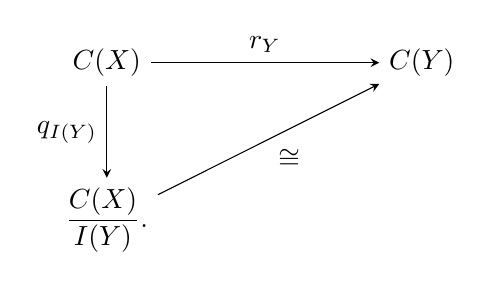
\begin{tikzpicture}[>=stealth]

        \node (CX) at (0,2) {$C(X)$};
        \node (CY) at (4,2) {$C(Y)$};
        \node (Q)  at (0,0) {$\displaystyle \frac{C(X)}{I(Y)}.$};
        
        \draw[->] (CX) -- node[above] {$r_Y$} (CY);
        
        \draw[->] (CX) -- node[left] {$q_{I(Y)}$} (Q);
        
        \draw[->] (Q) -- node[below right] {$\cong$} (CY);
        
        \end{tikzpicture}    
\end{equation}
S tem smo dokazali naslednje.
\begin{trditev}\label{trd:aux}
    Naj bo $\mathcal{S} \subseteq C(X) = C^*(\mathcal{S})$ operatorski sistem.
    Zaprta množica $Y \subseteq X$ je robna za $\mathcal{S}$
    natanko tedaj, ko je zožitev kvocientne preslikave $q_{I(Y)}: C(X) \to \quot{C(X)}{I(Y)}$ na $\mathcal{S}$ povsem izometrija.
\end{trditev}

To vodi do naslednje definicije.

\begin{definicija}\label{def:2.1}
    Naj bo $\mathcal{S} \subseteq C^*(\mathcal{S})$ operatorski sistem.
    Zaprt ideal $I \subseteq C^*(\mathcal{S})$ je \emph{robni ideal} za $\mathcal{S}$,
    če je zožitev kanonične kvocientne preslikave
    $q_I : C^*(\mathcal{S}) \to \quot{C^*(\mathcal{S})}{I}$
    na $\mathcal{S}$ povsem izometrija.
    Robnemu idealu pravimo \emph{ideal Šilova}, če vsebuje vse ostale robne ideale.
\end{definicija}

\begin{zgled}
    Če je $Y \subseteq X$ rob Šilova za operatorski sistem $\mathcal{S} \subseteq C(X) = C^*(\mathcal{S})$,
    potem je 
    $$I(Y) = \{f \in C(X)\ |\ f|_{Y} = 0\}$$
    njegov ideal Šilova.
\end{zgled}

Vsak robni ideal $I \subseteq C^*(\mathcal{S})$ inducira $C^*$-pokritje
$$q_I |_{\mathcal{S}}: \mathcal{S} \to \quot{C^*(\mathcal{S})}{I},$$
pri čemer je $q_I : \mathcal{C^*(\mathcal{S})} \to \quot{C^*(\mathcal{S})}{I}$ morfizem med $C^*$-pokritjema
$\mathcal{S} \hookrightarrow C^*(\mathcal{S})$ in $q_I |_{\mathcal{S}}$.
\begin{equation*}
    \begin{tikzpicture}[>=stealth, node distance=3cm]

        \node (S) at (0,2) {$\mathcal{S}$};
        \node (A) at (4,2) {$C^*(\mathcal{S})$};
        \node (Q) at (4,0) {$\frac{C^*(\mathcal{S})}{I}$.};
        
        % top arrow (unlabeled)
        \draw[{Hooks[right]}->]  (S) -- (A);
        
        % left diagonal arrow
        \draw[->] (S) -- node[left] {$q_I |_{\mathcal{S}}$} (Q);
        
        % right vertical arrow
        \draw[->] (A) -- node[right] {$q_I$} (Q);
        
    \end{tikzpicture}    
\end{equation*}
Ideal Šilova za $\mathcal{S}$ inducira najmanjše $C^*$-pokritje: $C^*$-ogrinjačo.

\begin{izrek}\label{izr:aux2}
    Za vsak operatorski sistem $\mathcal{S} \subseteq C^*(\mathcal{S})$ obstaja ideal Šilova $I \subseteq C^*(\mathcal{S})$
    in $q_I \big|_{\mathcal{S}}: \mathcal{S} \to \quot{C^*(\mathcal{S})}{I}$ je $C^*$-ogrinjača.
\end{izrek}

\begin{dokaz}
    Naj bo $i: \mathcal{S} \to C^* _{\env} (\mathcal{S})$ $C^*$-ogrinjača za $\mathcal{S}$.
    Po univerzalni lastnosti obstaja $*$-homomorfizem
    $\pi: C^*(\mathcal{S}) \to C_{\env} ^* (\mathcal{S})$, tako da je $\pi|_{\mathcal{S}} = i$.
    Dokazujemo, da je $I := \ker \pi$ ideal Šilova, torej da je zožitev kvocientne projekcije 
    $q_{I} : C^* (\mathcal{S}) \to \quot{C^* (\mathcal{S})}{I}$ na $\mathcal{S}$ povsem izometrija.
    Ker je $\pi: C^*(\mathcal{S}) \to C_{\env} ^* (\mathcal{S})$ surjektiven $*$-homomorfizem, je
    $$\overline{\pi}: \quot{C^*(\mathcal{S})}{I} \to C_{\env} ^* (\mathcal{S}),\quad a + \ker \pi \mapsto \pi (a)$$
    izometrični $*$-izomorfizem. Od tod sledi, da je 
    $$q_I |_{\mathcal{S}} = \overline{\pi}^{-1} \circ i: \mathcal{S} \to \quot{C^*(\mathcal{S})}{I}$$
    povsem izometrična preslikava, zato je $I$ robni ideal.
    
    Naj bo sedaj 
    $J \subseteq C^*(\mathcal{S})$ nek drug robni ideal in 
    $q_{J}: C^*(\mathcal{S}) \to \quot{C^*(\mathcal{S})}{J}$ njegova kanonična kvocientna projekcija,
    tako da je $q_J |_{\mathcal{S}}: \mathcal{S} \to \quot{C^*(\mathcal{S})}{J}$ $C^*$-pokritje za $\mathcal{S}$.
    Tedaj obstaja $*$-homomorfizem $\rho: \quot{C^*(\mathcal{S})}{J} \to C_{\env} ^* (\mathcal{S})$ iz univerzalne lastnosti, tako da velja 
    $\rho \circ q_J |_{\mathcal{S}} = i$. Po enoličnosti iz univerzalne lastnosti je $\rho \circ q_J = \pi$, zato 
    $J = \ker q_J \subseteq \ker \pi = I$.
\end{dokaz}


\begin{comment}
\begin{posledica}
    Za operatorski sistem $\mathcal{S} \subseteq M_n (C(X)) = C^*(\mathcal{S})$ 
    obstaja najmanjši zaprt podprostor $Y \subseteq X$, tako da vsaka matrika $A (x) = [a_{ij} (x)]_{i, j} \in \mathcal{S}$
    doseže svoj maksimum (v normi) na $Y$. 
\end{posledica}

\begin{dokaz}
    Znano dejstvo iz algebre je (DOPOLNI), da je za poljuben kolobar z enico $R$ vsak ideal $M_n (R)$
    oblike $M_n (I)$, kjer je $I$ ideal v $R$. 
    To pomeni, da so vsi zaprti ideali v $M_n (C(X))$ oblike $M_n (I(Y))$, kjer je $Y \subseteq X$ zaprta podmnožica.
    $$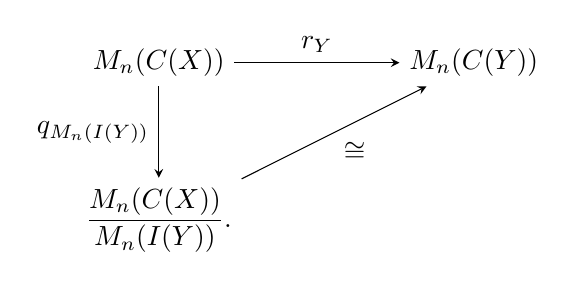
\begin{tikzpicture}[>=stealth]

        \node (CX) at (0,2) {$M_n (C(X))$};
        \node (CY) at (4,2) {$M_n (C(Y))$};
        \node (Q)  at (0,0) {$\displaystyle \frac{M_n(C(X))}{M_n (I(Y))}.$};
        
        \draw[->] (CX) -- node[above] {$r_Y$} (CY);
        
        \draw[->] (CX) -- node[left] {$q_{M_n (I(Y))}$} (Q);
        
        \draw[->] (Q) -- node[below right] {$\cong$} (CY);
        
        \end{tikzpicture}$$

    Po prejšnjem izreku za $\mathcal{S}$ obstaja ideal Šilova $I \subseteq M_n (C(X))$.

    To pomeni, da imamo bijektivno korespondenco med zaprtimi množicami v $X$ 
    in zaprtimi ideali v $M_n (C(X))$. V posebnem obstaja zaprta množica $Y \subseteq X$, tako da je 
    $I = M_n (C(Y))$. Od tod pa sledi, da je $Y$ najmanjša zaprta množica v $X$, tako da je 
    $$r_Y : M_n (C(X)) \to M_n (C(Y)),\quad [a_{ij}]_{i, j} \mapsto [a_{ij} |_Y ]_{i, j}$$
    izometrija.
\end{dokaz}
\end{comment}

\begin{posledica}[Šilov]
    Če je $\mathcal{S} \subseteq C(X) = C^*(\mathcal{S})$ operatorski sistem, potem obstaja njegov rob Šilova $Y$
    in $r_Y |_{\mathcal{S}}: \mathcal{S} \to C(Y)$ je njegova $C^*$-ogrinjača.
\end{posledica}

\begin{dokaz}
    Po izreku \ref{izr:2.3} obstaja ideal Šilova za $\mathcal{S}$, ki mora po lemi \ref{lem:aux} biti oblike 
    $$I(Y) = \{f \in C(X)\ |\ f|_Y = 0\}$$ za neko zaprto podmnožico $Y \subseteq X$. 
    Po trditvi \ref{trd:aux} je $Y$ rob Šilova za $\mathcal{S}$.    
    Zadnji stavek potem sledi iz izreka \ref{izr:aux2} in diagrama \eqref{eq:aux}.
\end{dokaz}

\begin{zgled}
    Oglejmo si ponovno operatorski sistem 
    $\mathcal{S} = \C[z] + \C[z]^* \subseteq C(\overline{\D})$
    iz zgleda \ref{zgl:2.1}. 
    Dokazali smo že, da je $\T$ njegov rob Šilova, zato je 
    $$I(\T) = \{f \in C(\overline{\D})\}$$ 
    njegov ideal Šilova ter
    $r_Y |_{\mathcal{S}}: \mathcal{S} \to C(\T)$ njegova $C^*$-ogrinjača.
\end{zgled}

Naslednji zgled je podrobneje obravnavan v \cite{connes2021}.

\begin{zgled}[Connes-van Suijlekom] \label{zgl:2.2}
    Označimo s $\mathcal{T}^{(n)}$ \emph{Toeplitzov operatorski sistem}, ki ga sestavljajo \emph{Toeplitzove matrike}  
    $$\begin{bmatrix}
        a_0 & a_{-1} & a_{-2} & \cdots & a_{-n}\\
        a_{1} & a_0 & a_{-1} & \ddots & \vdots\\
        a_{2} & a_1 & a_0 & \ddots & a_{-2}\\
        \vdots & \ddots & \ddots & \ddots & a_{-1}\\
        a_{n} & \cdots & a_{2} & a_{1} & a_0
    \end{bmatrix} \in M_n (\C)$$
    
    Najprej skicirajmo, zakaj velja $C^*(\mathcal{T}^{(n)}) = M_n (\C)$.
    Označimo matriko $S = \sum_{k = 1} ^n E_{k+1, k} \in M_n (\C)$, ki je Toeplitzova matrika za $a_{1} = 1$ in $a_k = 0, k \neq 1$.
    Potem je $S S^* = I - E_{11}$, zato je $E_{11} \in C^*(\mathcal{T}^{(n)})$.
    Z indukcijo dokažemo, da so vse matrike oblike $E_{kk}$ v $C^*(\mathcal{T}^{(n)})$:
    če je namreč $E_{k - 1, k - 1} \in C^*(\mathcal{T}^{(n)})$, potem enako velja tudi za $E_{k, k - 1} = S E_{k - 1, k - 1}$
    in $E_{k-1, k} = E_{k, k - 1}^*$ ter posledično $E_{kk} = E_{k, k - 1} E_{k - 1, k}$.
    Sedaj, ko imamo vse diagonalne matrične enote, dobimo tudi 
    $E_{k + i, k} = S^i E_{k, k}$ in $E_{k, k + i} = E_{k + i, k}^*$.

    Po izreku \ref{izr:2.3} potem obstaja njegov ideal Šilova $I \subseteq M_n (\C)$.
    Ker pa je $M_n (\C)$ enostaven kolobar, je $I = (0)$ in $C^* _{\env} (\mathcal{T}^{(n)}) = \quot{M_n (\C)}{I} = M_n (\C)$.
\end{zgled}

Toeplitzove matrike iz prejšnjega zgleda bomo v naslednjem zgledu posplošili do neskončno dimenzionalnih matrik nad Hilbertovim prostorom $\ell^2 (\Z_+)$.
Dokaze bomo izpustili in se zgolj sklicali na knjigo \cite{arveson2002}, v kateri je ta material podrobneje obravnavan.

\begin{zgled}\label{zgl:2.3}
    Oglejmo si operatorje $T \in \mathcal{B}(\ell^2 (\Z_+))$, ki imajo glede na standardno bazo $\{e_n\}_{n \in \Z}$ matriko oblike 
    \begin{equation}\label{eq:aux2}
        \begin{bmatrix}
        a_0 & a_{-1} & a_{-2} & \cdots \\
        a_{1} & a_0 & a_{-1} & \cdots \\
        a_{2} & a_1 & a_0 & \cdots \\
        \vdots & \vdots & \vdots & \ddots
    \end{bmatrix}\end{equation}
    Izkaže se, da za takšne operatorje obstaja zelo lepa karakterizacija s t.i.~\emph{Toeplitzovimi operatorji}.

    Začnemo s prostorom $L^2 (\T, m)$, kjer je $m$ normalizirana Lebesgueova mera na $\T$.
    Iz Fouriereve teorije vemo, da funkcije $\{z^n\}_{n \in \Z}$ tvorijo ortonormirano bazo Hilbertovega prostora $L^2 (\T, m)$.
    Sedaj definiramo \emph{Hardyjev prostor} $$H^2 := \overline{\lin\{1, z, z^2, \dots\}} \subseteq L^2 (\T, m).$$
    To je torej prostor $L^2$ funkcij $f$ na $\T$, ki imajo Fourierovo vrsto oblike 
    $$f(e^{i\theta}) \sim \sum_{n = 0} ^\infty a_n e^{i n \theta}.$$
    Ker funkcije $\{z^n\}_{n \in \Z_+}$ tvorijo ortonormirano bazo Hilbertovega prostora $H^2$,
    lahko $H^2$ na očiten način identificiramo s prostorom $\ell^2 (\Z_+)$. Nadalje lahko za vsako funkcijo $f \in L^\infty (\T, m)$
    definiramo operator 
    $$M_f \in \mathcal{B}(L^2 (\T, m)),\quad M_f (g) = fg$$
    in Toeplitzov operator 
    $$T_f \in \mathcal{B} (H^2),\quad T_f = P_{H^2} M_f |_{H^2}.$$
    Po izreku \cite[Theorem 4.2.4, str. 108]{arveson2002} so operatorji $T \in \mathcal{B}(\ell^2 (\Z_+))$ oblike \eqref{eq:aux2}
    natanko operatorji $T_f$ za $f \in L^\infty (\T, m)$, pri čemer je $\| T_f \| = \| f\|_\infty$.
    Z drugimi besedami: formalna Toeplitzova matrika 
    $$\begin{bmatrix}
        a_0 & a_{-1} & a_{-2} & \cdots \\
        a_{1} & a_0 & a_{-1} & \cdots \\
        a_{2} & a_1 & a_0 & \cdots \\
        \vdots & \vdots & \vdots & \ddots
    \end{bmatrix}$$
    je matrika omejenega operatorja natanko tedaj, ko obstaja funkcija $f \in L^\infty (\T, m)$,
    ki ima Fourierevo vrsto $f(e^{i\theta}) \sim \sum_{n = -\infty} ^\infty a_n e^{i n \theta}$.

    Posebno lepa teorija je za Toeplitzove operatorje \emph{z zveznim simbolom}:
    $$\mathcal{T}(C(\T)) := \{T_f\ |\ f \in C(\T)\}.$$
    Označimo $S := T_z \in \mathcal{T} (C(\T))$, ki ustreza operatorju desnega premika na $\ell^2 (\Z_+)$,
    torej $S e_n = e_{n + 1}.$ Operator $S$ generira algebro $C^*(S)$, ki je izjemnega pomena v funkcionalni analizi: rečemo ji \emph{Toeplitzova algebra}. 
    Izrek \cite[Theorem 4.3.2, str. 111]{arveson2002} nam pove, da je Toeplitzova algebra oblike 
    $$C^*(S) = \{T_f + K\ |\ f \in C(\T),\ {K \in \mathcal{K}(H^2)}\},$$
    pri čemer s $\mathcal{K}(H^2)$ označujemo kompaktne operatorje na $H^2$.
    Izrek nam pove še več: vsak element Toeplitzove algebre lahko na enoličen način razpišemo kot $T_f + K$.

    Sedaj lahko določimo ideal Šilova za $\mathcal{T}(C(\T))$. Najprej dokažimo,
    da je to sploh operatorski sistem. Hitro lahko preverimo, da velja 
    $$T_{\alpha f + \beta g} = \alpha T_f + \beta T_g,\quad T_{f} ^* = T_{\overline{f}},$$
    zato je $\mathcal{T}(C(\T))$ vektorski prostor, ki je zaprt za adjungacijo in vsebuje $1 = T_1.$
    Iz prejšnjega odstavka nato takoj sledi, da $\mathcal{T}(C(\T))$ generira Toeplitzovo algebro $C^*(S)$.
    Dokazujemo, da je njegov ideal Šilova kar $\mathcal{K}(H^2) \subseteq C^*(S)$.
    
    Znano je namreč, da kompaktni operatorji tvorijo zaprt ideal v algebri operatorjev na Hilbertovem prostoru.
    Za začetek dokažimo, da je $\mathcal{K}({H^2})$ robni ideal za $\mathcal{T}(C(\T))$.
    Ker ima vsak element v $C^*(S)$ enoličen zapis oblike $T_f + K$, lahko definiramo preslikavo
    $$\varphi: C^*(S) \to C(\T),\quad T_f + K \mapsto f.$$
    Enostavno je preveriti, da je $\varphi$ $*$-homomorfizem in $\ker \varphi = \mathcal{K}(H^2)$, zato imamo komutativni diagram  
    \begin{equation*}
        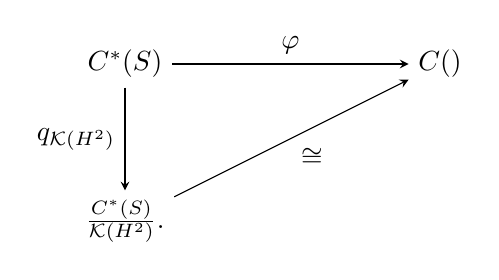
\begin{tikzpicture}[>=stealth, node distance=3cm]
    
            \node (S) at (0,2) {$C^*(S)$};
            \node (A) at (4,2) {$C(\T)$};
            \node (Q) at (0,0) {$\frac{C^*({S})}{\mathcal{K}(H^2)}$.};
            
            % top arrow (unlabeled)
            \draw[->]  (S) -- node[above] {$\varphi$} (A);
            
            % left diagonal arrow
            \draw[->] (S) -- node[left] {$q_{\mathcal{K}(H^2)}$} (Q);
            
            % right vertical arrow
            \draw[->] (Q) -- node[below right] {$\cong $} (A);
            
        \end{tikzpicture}    
    \end{equation*}
    Za vsak $f \in C(\T)$
    je $$\| \varphi(T_f) \| = \| f\| = \| T_f\|,$$
    zato je $\varphi|_{\mathcal{T}(C(\T))}: \mathcal{T}(C(\T)) \to C(\T)$ enotska izometrija in posledično povsem skrčitev.
    Enako velja tudi za njen inverz, zato je $\varphi|_{\mathcal{T}(C(\T))}: \mathcal{T}(C(\T)) \to C(\T)$ enotska povsem izometrija.
    Po zgornjem diagramu je tudi $q_{\mathcal{K}(H^2)} |_{\mathcal{T}(C(\T))}: \mathcal{T}(C(\T)) \to \quot{C^*({S})}{\mathcal{K}(H^2)}$
    povsem izometrija in $\mathcal{K}(H^2)$ je robni ideal. 
    Dokažimo še, da je tudi ideal Šilova.
    
    Vzemimo nek poljuben ideal $I \supseteq \mathcal{K}(H^2)$ v $C^*(S)$.
    Potem mora $I$ vsebovati nek Toeplitzov operator $T_f$, kjer je $f \in C(\T)$ neničelna funkcija.
    To pa pomeni, da $q_I |_{\mathcal{T}(C(\T))}: \mathcal{T}(C(\T)) \to \quot{C^*(S)}{I}$ uniči $T_f \neq 0$,
    zato ne more biti povsem izometrija.
\end{zgled}